\section{Evaluating the code}

In this section we will show how the posterior parameter distributions that we can generate from the output
of our nested sampling code compare to evaluating them with a previous implementation of the analysis code
\citep[\lppe used in e.g.][]{2014ApJ...785..119A} using a (generally inefficient) MCMC algorithm and over a grid in parameters.
We will show comparisons of the codes in two different regimes: no signal is present in the data, and an obvious signal is
present in the data. We do this using simulated data both containing purely Gaussian noise and containing simulated signals
added to Gaussian noise.

Using a selection of many simulated signals we also show how the odds comparing a signal model and a noise only model change with
signal-to-noise ratio, along with comparing coherent verses incoherent signals (for coherent simulated signal and incoherent simulations).
The simulations also allow us to evaluate the posterior probabilty distributions produced by the code using what is colloquially known,
in ground-based \gw parameter estimate circles at least, as ``P-P plots'' (see \S\ref{sec:ppplots})

\subsection{Code comparison}

In each of the tests below we will be running our code (\lppen) using the default proposal distributions discussed in \S\ref{sec:proposals}
and with the number of live points fixed to be 2048. We will also assume a source at a fixed sky position and that the signal model is purely
that for the $l=m=2$ harmonic (Equation~\ref{eq:h2f}), and that we work in terms of the signal amplitude $h_0$ and signal phase
$\Phi_{22}^C$ (this is for consistency with the old code which uses $\Phi_{22}^C$ rather than $\phi_0$, which we have earlier defined as the
rotational phase). The simulated data in all cases 
will be generated as the complex heterodyned
time series sampled once per minute. When comparisons between the current code and previous codes are 
made we run the current code in a way that splits datasets into 30 point chunks, rather than using the algorithm described in \S\ref{sec:splitting},
as this makes it consistent with the old code (\lppe). We also purely use the uniform prior ranges for the amplitude parameter to be
consistent between codes.

\subsubsection{Simulated noise}\label{sec:simnoise}

An initial test of the code is whether the output posterior probability distributions match those produced when evaluating the
posterior over a fixed grid in the four-dimensional parameter space of $\vec{\theta} = \{h_0, \cos{\iota}, \psi, \phi_{22}^C\}$, when
using purely Gaussian noise.\footnote{It is worth noting that in many of these tests the polarisation angle prior covers $-\pi/4$ to $\pi/4$
rather than the 0 to $\pi/2$ range given in, e.g., \citet{2015MNRAS.453.4399P} due to this being the range required by the older
parameter estimation MCMC code. Although this range is degenerate to rotations over $\pi/2$, so spans the same range of waveform models.}
A comparison of the marginalised posteriors for individual parameters, and pairs of parameters, are shown when using simulated data lasting
ten days from a single detector (in this case assumed to be the LIGO Hanford detector, H1) in Figure~\ref{fig:simnoise_single}.

\begin{figure}[!phtb]
\begin{center}
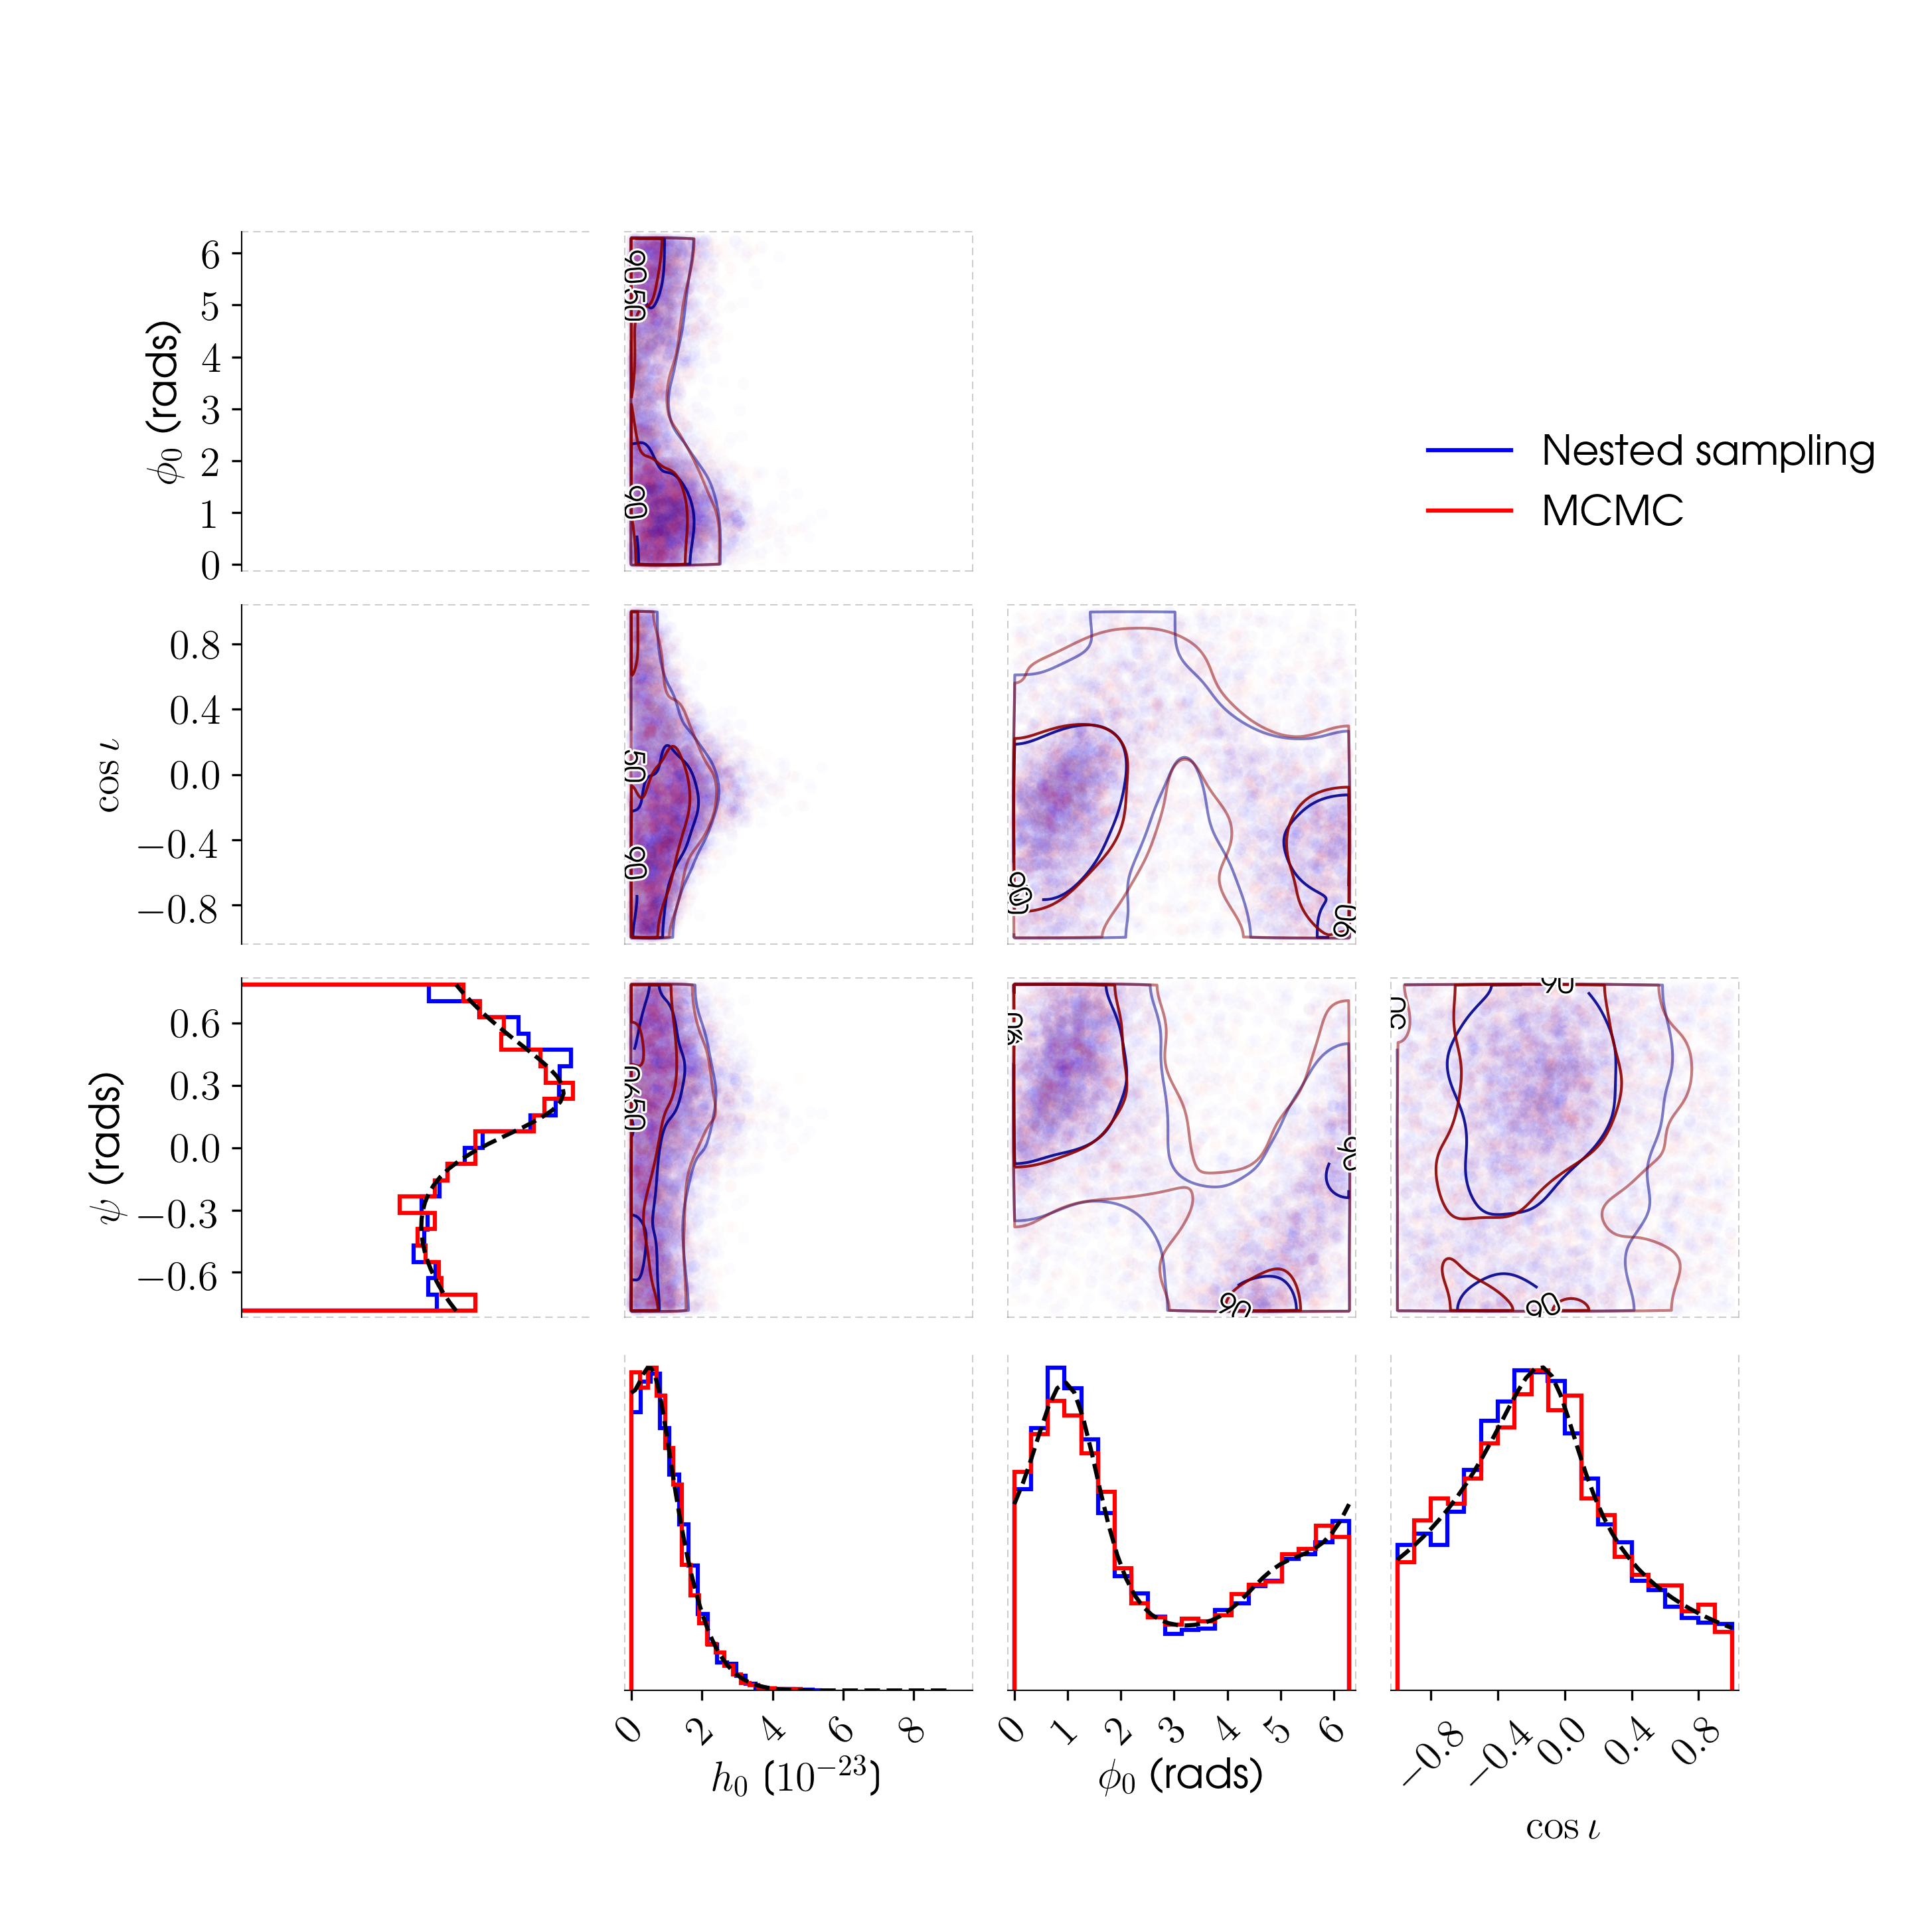
\includegraphics[width=1\columnwidth]{./figures/codeeval/simulations/noise/simulatednoisetest}
\caption{ \protect\label{fig:simnoise_single}
Marginalised one and two-dimensional posterior probability distributions
for the parameters $\{h_0, \cos{\iota}, \psi, \phi_0\}$
produced from the outputs of the nested sampling code \lppen, and the previous
code \lppe, when running on simulated Gaussian noise assumed from the LIGO H1 detector. The \lppe code was run with both an MCMC sampler mode and a grid-based
evaluation mode (shown as the black dashed line).
}
\end{center}
\end{figure}

It can be seen that the output posteriors look qualititavely consistent. However, we can also quantify some aspects of consistency by
comparing the evidence output from the nested sampling code with that estimated from the grid-based method from \lppe, the upper limits
on $h_0$ produced by the codes, and performing Kolmogorov-Smirnov consistency tests between the nested sampling posterior samples
and MCMC posterior samples (giving a $p$-value for the null hypothesis that the samples are from the same distributions).
These are shown in Table~\ref{tab:codeeval} and show very good consistency between the codes, although it should be noted that
these are for one particular run and some statistical fluctuations in the exact values for different runs are to be expected (see e.g.\
the variations in evidence values in \S\ref{sec:proposaltesting}).

A {\tt jupyter} notebook with this test can be found \href{https://github.com/mattpitkin/CW_nested_sampling_doc/blob/master/figures/codeeval/simulations/noise/SimulatedNoiseTestsPaper.ipynb}{here}.

\begin{table*}[hptb]
\caption{Consistency tests between outputs of the new code, \lppen, and the old code, \lppe, when running on simulated data
and searching over the four parameters $\{h_0, \cos{\iota}, \psi, \Phi_{22}^C\}$.\label{tab:codeeval}}
\begin{center}
\begin{tabular}{l c c | c c c c}
\hline
\multirow{2}{*}{Simulation} & \multirow{2}{*}{$\ln{\left(\frac{Z_{\text{nested}}}{Z_{\text{grid}}}\right)}$} & \multirow{2}{*}{$\frac{(h_0^{95\%})_{\text{nested}}}{(h_0^{95\%})_{\text{grid}}}$} & 
\multicolumn{4}{c}{K-S $p$-value} \\ \cline{4-7}
 &  &  & $p(h_0)$ & $p(\Phi_C^{22})$ & $p(\cos{\iota})$ & $p(\psi)$ \\                      
\hline
\hline
Noise (single detector)  & $-0.07$ & $1.009$ & 0.404 & 0.026 & 0.010 & 0.703 \\
Noise (two detectors)    & $-0.05$ & $0.992$ & 0.141 & 0.564 & 0.538 & 0.493 \\
Signal (single detector) & 0.245   & $1.004$ & 0.237 & 0.291 & 0.125 & 0.175 \\
Signal (two detectors)   & 0.240   & 0.991   & 0.722 & 0.052 & 0.067 & 0.032 \\
\hline
\end{tabular}
\end{center}
\end{table*}

We see a very similar situation, in terms of agreement between the codes, when running on simulated data assumed to be from two detectors (the LIGO
H1 and L1 sites) as shown in Figure~\ref{fig:simnoise_single} and the second line of Table~\ref{tab:codeeval}. A {\tt jupyter} notebook with this test
can be found \href{https://github.com/mattpitkin/CW_nested_sampling_doc/blob/master/figures/codeeval/simulations/noise_multidet/SimulatedNoiseTestsMultidetPaper.ipynb}{here}.

\begin{figure}[!phtb]
\begin{center}
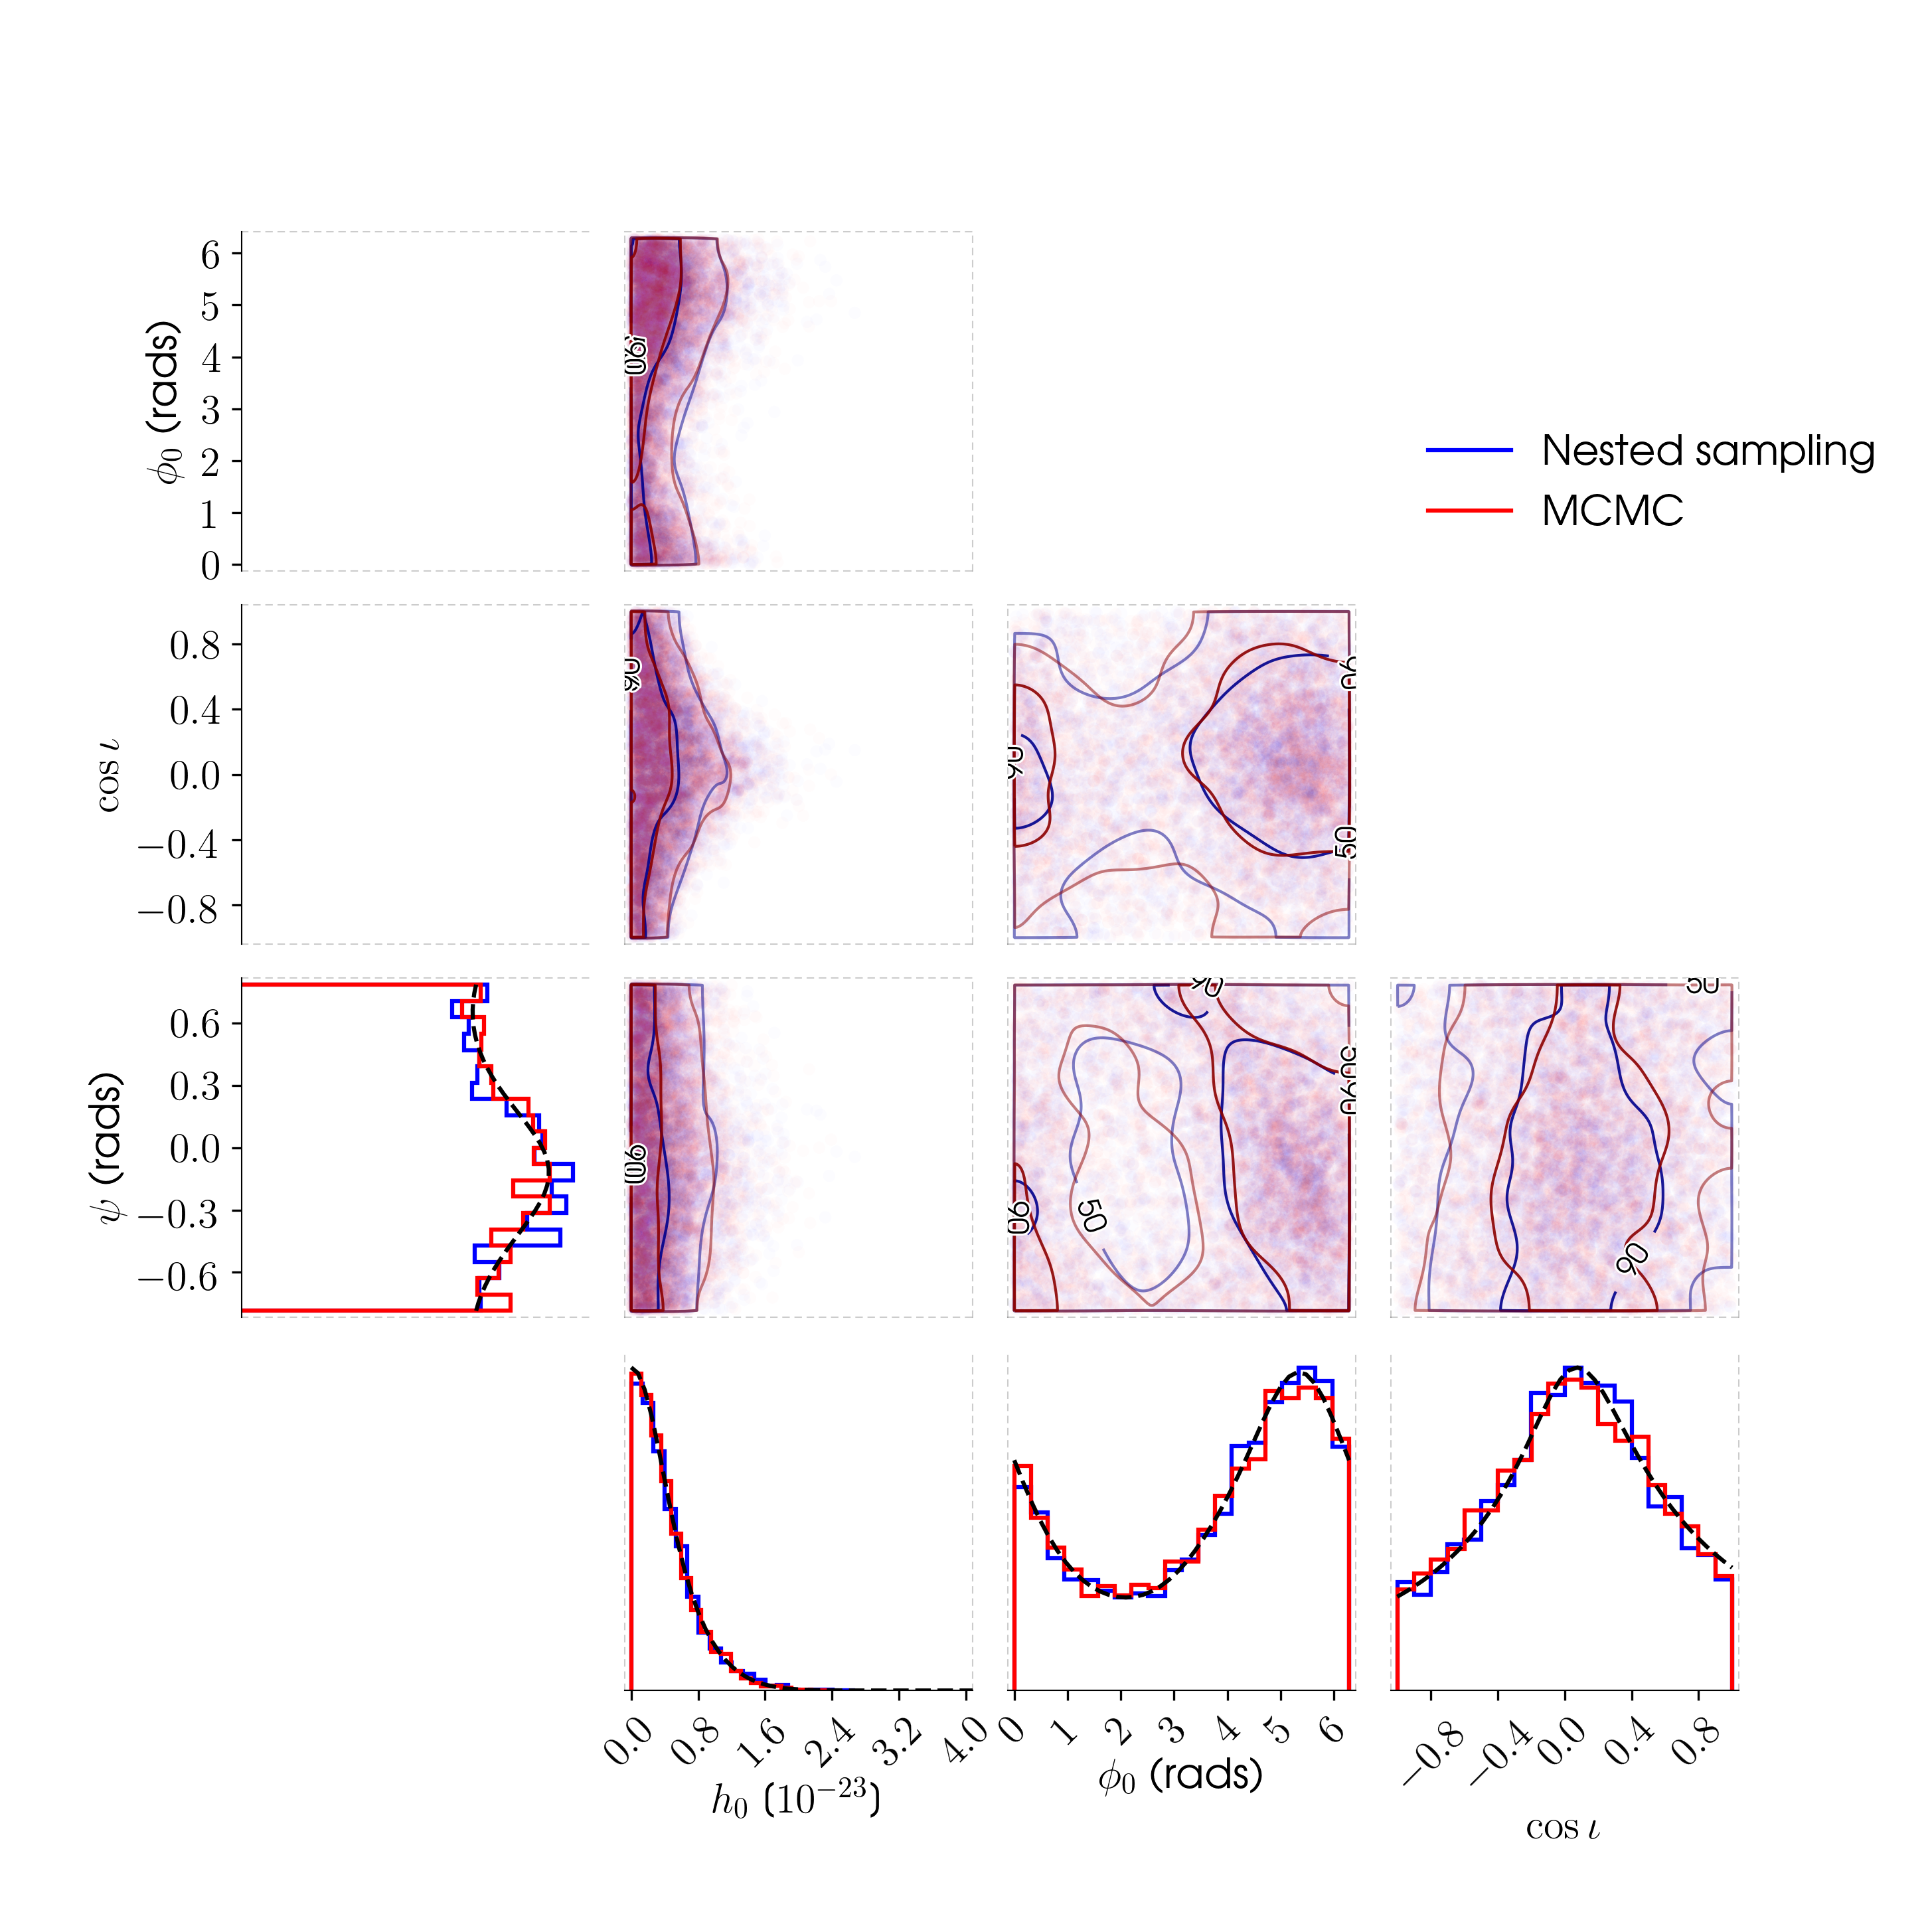
\includegraphics[width=1\columnwidth]{./figures/codeeval/simulations/noise_multidet/simulatednoisemultidettest}
\caption{ \protect\label{fig:simnoise_multi}
Marginalised one and two-dimensional posterior probability distributions
for the parameters $\{h_0, \cos{\iota}, \psi, \phi_0\}$
produced from the outputs of the nested sampling code \lppen, and the previous
code \lppe, when running on simulated Gaussian noise assumed from the LIGO H1 and
L1 detectors. The \lppe code was run with both an MCMC sampler mode and a grid-based
evaluation mode (shown as the black dashed line).
}
\end{center}
\end{figure}

The above tests using simulated noise and with searches covering the four standard unknown \gw parameter show that the code appears to
be working as expected, and is in agreement with our previously used code. However, more generally we can perform parameter estimation
over a larger number of signal parameters, and can again check for consistency with the previous code. We produce one day of Gaussian
noise for a single detector and search over the four \gw parameter with the same priors as before, but then also use a multi-variate Gaussian prior (\S\ref{sec:gaussianprior})
over the {\it phase} parameters: rotational frequency and first frequency derivative, and binary parameters of binary period, time of periastron, angle of
periastron and its first derivative, projected semi-major axis, and eccentricity ($\{f,\dot{f},P_{\text{b}}, T_0, \omega_0, \dot{\omega}_0, a\sin{i}, e\}$).
This gives a total of 12 parameters in the search. The multi-variate prior is defined such that all parameters are uncorrelated except, in this case,
the parameter pairs $[T_0, \omega_0]$ and $[P_{\text{b}}, \dot{\omega}_0]$ for which we use a very high correlation of $0.9999$ (we do not set them to
be fully correlated due to numerical issues inverting such matrices).

The one-and-two dimensional posteriors output for this case when run with both \lppe and \lppen can be seen in Figure~\ref{fig:noise_multiparam},
which also overlays the marginalised priors on top. It can be seen qualititavely that the codes are consistent\footnote{It is worth mentioning that in performing
these tests a bug was discovered in \lppe in which Equation~\ref{eq:deltaphi} was being applied with the wrong sign, leading to parameter estimates
having the wrong sign. However, this bug was fixed for the example shown here.} and for the {\it phase} parameter priors are recovered, except for
$\dot{f}$, which has some structure due to the specifics of the noise realisation. The Kolmogorov-Smirnov test $p$-values testing the null hypothesis
that the posterior samples from each code are drawn from the same distribution are shown in Table~\ref{tab:noisemultiks}, and suggest that the
distributions are consistent.

\begin{table*}[hptb]
\caption{Kolmogorov-Smirnov test $p$-values testing the null hypothesis that the samples output by \lppen and \lppe, when running on simulated
noise data and searching over the twelve parameters $\{h_0, \cos{\iota}, \psi, \Phi_{22}^C, f,\dot{f},P_{\text{b}}, T_0, \omega_0, \dot{\omega}_0, a\sin{i}, e\}$,
are drawn from the same distributions.\label{tab:noisemultiks}}
\begin{center}
\begin{tabular}{l | c c c c c c c c c c c c}
\hline
Parameter & $h_0$ & $\Phi_C^{22}$ & $\cos{\iota}$ & $\psi$ & $f$ & $\dot{f}$ & $P_{\text{b}}$ & $T_0$ & $\omega_0$ & $\dot{\omega}_0$ & $a\sin{i}$ & $e$ \\                      
\hline
\hline
$p$-value  & 0.13 & 0.04 & 0.78 & 0.23 & 0.44 & 0.26 & 0.85 & 0.28 & 0.29 & 0.86 & 0.52 & 0.28 \\
\hline
\end{tabular}
\end{center}
\end{table*}

\begin{figure*}[!phtb]
\begin{center}
\includegraphics[width=0.9\textwidth]{./figures/codeeval/simulations/noise_multiparam/noise_multiparam}
\caption{ \protect\label{fig:noise_multiparam}
Posterior probability distributions for multiple parameters using simulated noise.
}
\end{center}
\end{figure*}

\subsubsection{Simulated signals}\label{sec:simsignal}

The next test is checking how the codes compare when there is a signal present in the data. When generating the simulated signals we initially
assume that the signal's phase evolution is perfectly known and has been removed via the heterodyne described in \S\ref{sec:model}, and therefore
$\Delta\phi_2 = 0$ from Equation~\ref{eq:deltaphi}. As in \S\ref{sec:simnoise} then will search over the four-dimensional parameter space of
$\vec{\theta} = \{h_0, \cos{\iota}, \psi, \Phi_{22}^C\}$.

We create a simulated signal in the H1 detector spanning ten days of data with parameters ($h_0 = 6.2\ee{-23}$, $\Phi_{22}^C = 2.4$\,rad, $\cos{\iota} = 0.3$
and $\psi = 0.1$\,rad) that produce a signal-to-noise ratio of 8 when injected into
Gaussian noise. The posterior probability distributions estimated for the parameters (expressed as offsets from the assumed heterodyne parameter values) are
shown in Figure~\ref{fig:simsignal_single}, which show consistency
between the old and new codes and with the injected signal parameters. The quantitative consistency between the codes can be seen in Table~\ref{tab:codeeval},
where is should be noted that the evidence ratio between the codes is larger than statistical uncertainty would expect, although the fractional difference between
the values ($\lesssim 1\%$) is still small enough to not greatly effect conclusions drawn from either values if used in model selection.

\begin{figure}[!phtb]
\begin{center}
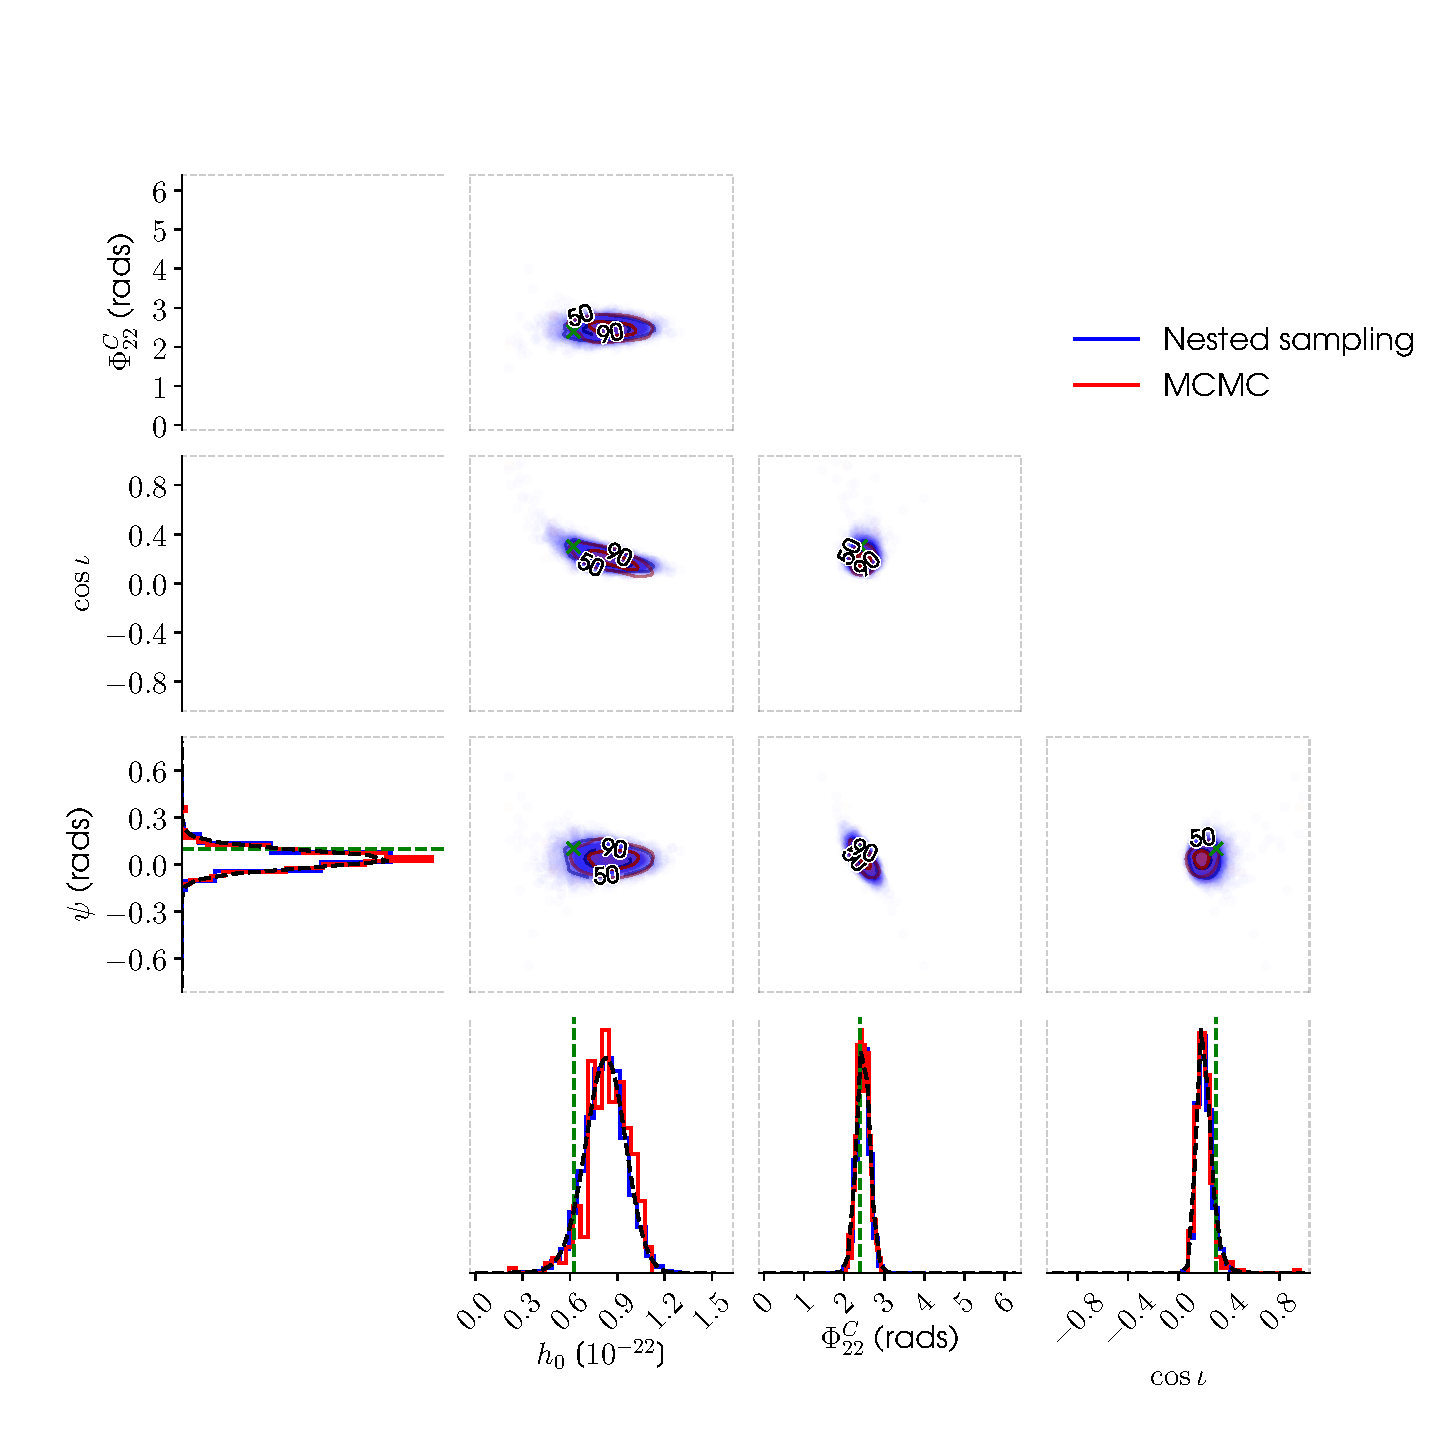
\includegraphics[width=1\columnwidth]{./figures/codeeval/simulations/signal/simulatedsignaltest}
\caption{ \protect\label{fig:simsignal_single}
Marginalised one and two-dimensional posterior probability distributions
for the parameters $\{h_0, \cos{\iota}, \psi, \Phi_{22}^C\}$
produced from the outputs of the nested sampling code \lppen, and the previous
code \lppe, when running on simulated data containing Gaussian noise and a signal 
(of SNR 8) assumed from the LIGO H1 detector. The \lppe code was run with both an MCMC sampler mode and a grid-based
evaluation mode (shown as the black dashed line).
}
\end{center}
\end{figure}

Similarly, using a signal with a coherent multi-detector signal-to-noise ratio of 8 (for the same parameters as above except with $h_0 = 3.5\ee{-23}$) when
simulated and injected into Gaussian noise for two detectors (H1
and L1) we see the posteriors shown in Figure~\ref{fig:simsignal_multi}, and consistency checks in Table~\ref{tab:codeeval}.

\begin{figure}[!phtb]
\begin{center}
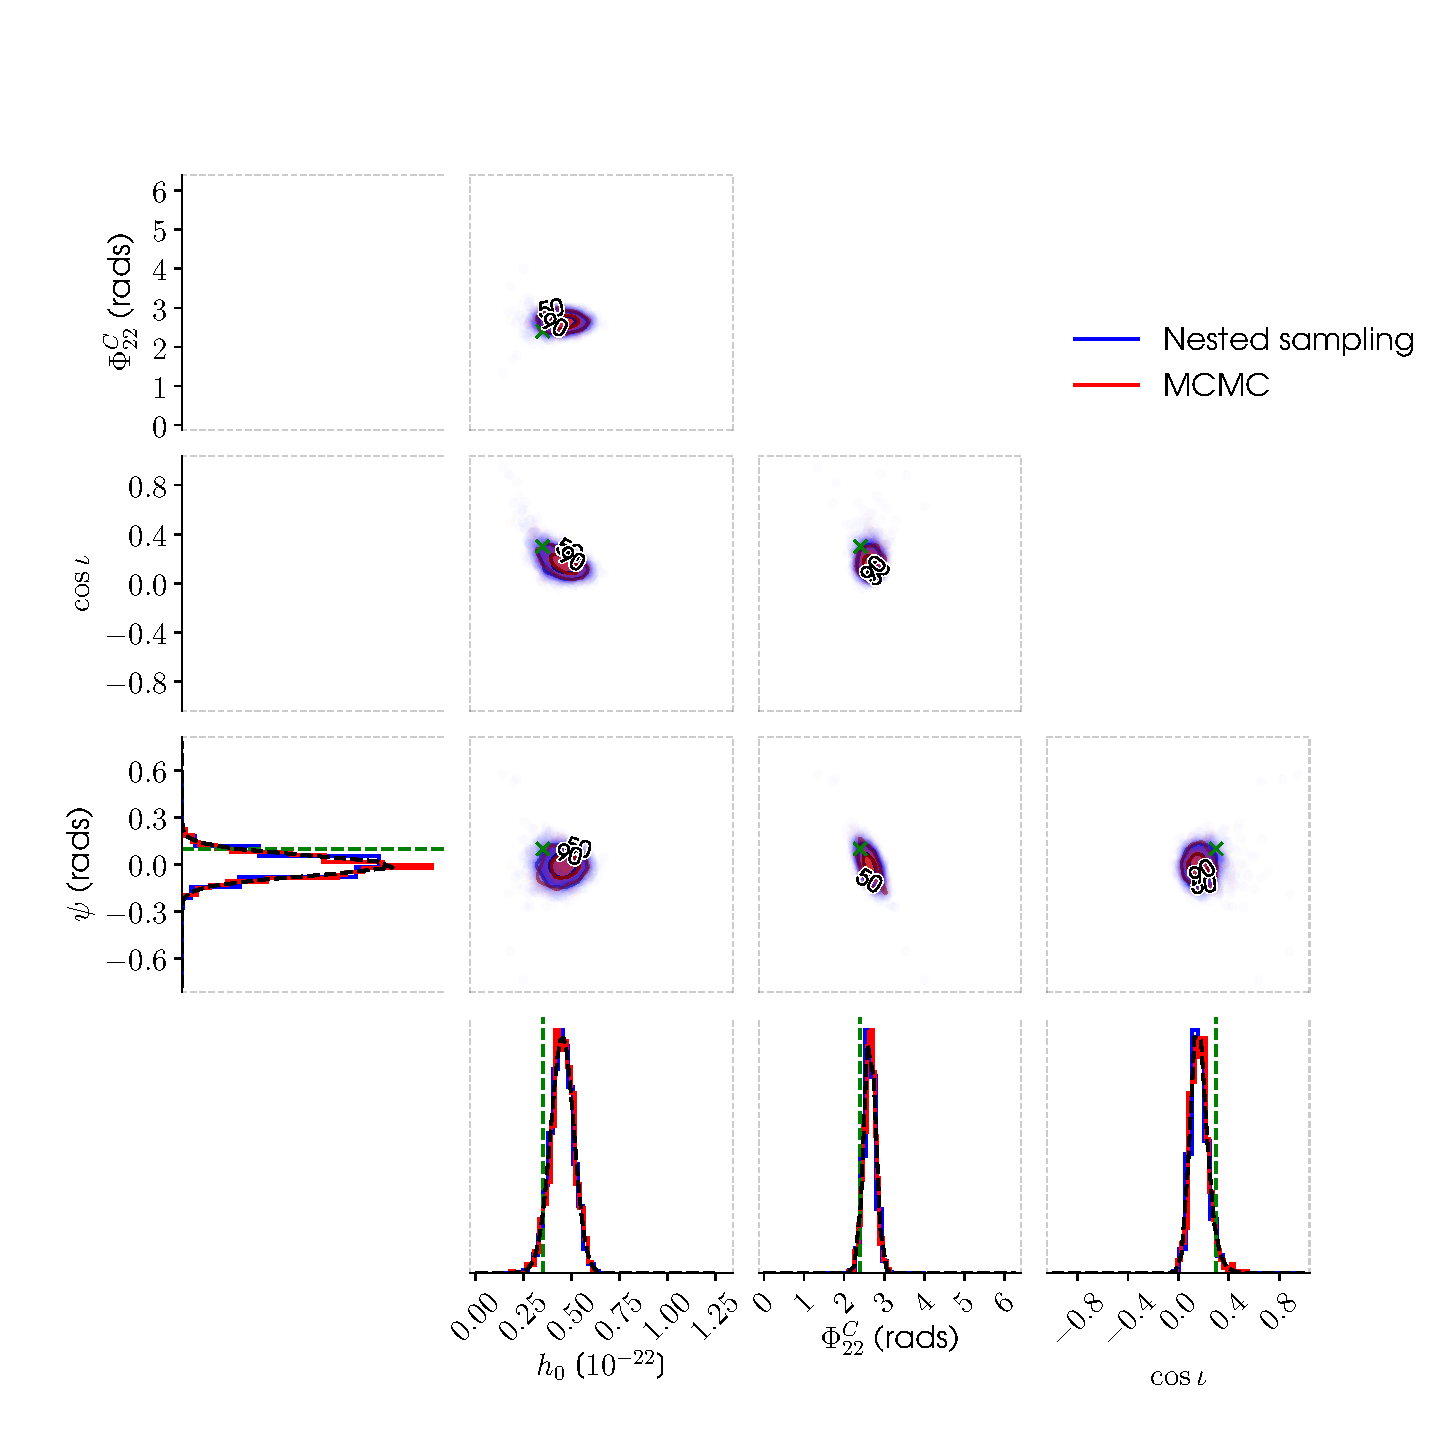
\includegraphics[width=1\columnwidth]{./figures/codeeval/simulations/signal_multidet/simulatedsignalmultitest}
\caption{ \protect\label{fig:simsignal_multi}
Marginalised one and two-dimensional posterior probability distributions
for the parameters $\{h_0, \cos{\iota}, \psi, \phi_0\}$
produced from the outputs of the nested sampling code \lppen, and the previous
code \lppe, when running on simulated data containing Gaussian noise and a signal 
(of coherent multi-detector SNR 8) assumed from the LIGO H1 and L1 detectors. The \lppe code was run with both an MCMC sampler mode and a grid-based
evaluation mode (shown as the black dashed line).
}
\end{center}
\end{figure}

The notebooks for the above two tests can be found \href{https://github.com/mattpitkin/CW_nested_sampling_doc/blob/master/figures/codeeval/simulations/signal/SimulatedSignalTestsPaper.ipynb}{here} and 
\href{https://github.com/mattpitkin/CW_nested_sampling_doc/blob/master/figures/codeeval/simulations/signal_multidet/SimulatedSignalMultidetTestsPaper.ipynb}{here}.

A set of simulated signals with sky location and orbital parameters set to those of the Low-mass X-ray binary Sco X-1 were injected into
Gaussian noise for the study in \citet{2015PhRvD..92b3006M}. As a test of our code when recovering a signal from a source in a binary system
we have recovered one of these signals using approximately 1.4 days of simulated data. We have purposely performed the heterodyne data processing stage
with values of several of the phase parameters ($f_0$, $\alpha$, $T_0$, $a\sin{i}$ and $P_{\text{b}}$) set to {\it not} match the known simulated signal
values. Therefore, to recover the signal, in addition to the four \gw parameters we have had to allow the code to search over these extra parameters.
For these additional parameters Gaussian priors were used, with the prior means set to be the parameter values used for heterodyning (not those for
the actual signal), with standard devaitions wide enough to encompass the true signal values. For $h_0$ a Fermi-Dirac prior was used, whilst the other
angle parameters used priors covering their minimal allowed ranges. The recovered signal posterior distributions can be seen
in Figure~\ref{fig:scox1_inj}, which show that the true parameters are correctly recovered (the plot show recovered phase parameters as offsets from
the heterodyne parameter values, i.e.\ the centres of the Gaussian priors). It can be seen that for $f_0$ and $P_{\text{b}}$ the posteriors contain the
correct value, but are peaked well away from the value used for heterodyning (which would be a zero in the plots), showing the codes ability to explore
the prior space in these parameters. The one-dimensional marginal distribution for $\phi_0$ spans the full prior range, however, this is due to it being
highly correlated with $f_0$, and, although not visible on the plot, this very strong correlation is present in the two-dimensional posterior for these
parameters. Finally, for $\alpha$ and $T_0$ it can be seen that the posteriors just fill the prior ranges as the data give not additional information
about these parameters. For completeness, we find that the the signal was recovered with SNRs of $\sim 20$ in both H1 and L1 individually, with a coherent
SNR of $\sim 28$, and odds values for the multi-detector analysis of $\log{}_{10}\left(\mathcal{O}_{\text{S}/\text{N}}\right) = 152$
and $\log{}_{10}\left(\mathcal{O}_{\text{S}/\text{I}}\right) = 7.8$.

\begin{figure*}[!phtb]
\begin{center}
\includegraphics[width=0.9\textwidth]{./figures/codeeval/simulations/scox1_inj/scox1_inj}
\caption{ \protect\label{fig:scox1_inj}
Marginalised posterior plots for the recovered parameters of a simulated binary signals (with binary parameters
similar to those of Sco X-1) using simulated LIGO H1 (red) and L1 (green) data, including a joint detector analysis
(grey). The location of the simulated signal parameters are marked with a vertical black dash line on the, or black
cross. The priors used for each parameter are shown as the dark magenta dashed lines.
}
\end{center}
\end{figure*}

\subsubsection{Results evaluation}\label{sec:reseval}

The above results have shown good qualititive, and quantitative, agreement between the old and new codes for individual cases, but it is also useful
to see how they compare for a large number of noise realisations when assessing two important quantities: the 95\% upper limit on \gw amplitude $h_0$,
and the signal model evidence. It is also useful to see how these compare as a function of the number of live points used by the code. To this end we
have choosen numbers of live points from 256 to 16384, increasing in a power of two for each step, and for each number generated 500 reaslisations of
complex Gaussian noise with 1440 points over one day. Choosing a random source sky location for each realisation, and using uniform priors for the
parameters $h_0$, $\cos{\iota}$, $\Phi_{22}^C$ and $\psi$, we have performed parameter estimation using both \lppen and \lppe in its grid-based mode.
For \lppe the integrals required for calculating the signal evidence and 95\% upper limit on $h_0$ are performed using the trapezium rule, whilst
for the output of \lppen the upper limit has been calculated used a greedy-binning approach bounded from zero. This assessment is very similar to what
we did in \S\ref{sec:proposaltesting}, but has not just used a fixed Gaussian likelihood function in each case. We will make the assumption that the
grid-based results are a representation of the true values for the evidence and upper limit, however, it should be noted that there will in fact be
errors (and potentially biases) from the trapezium rule approximation.

In Figure~\ref{fig:nest_evs} we see a comparison between the signal evidences evaluation using nested sampling and the trapezium rule. The left-hand
axis shows the logarithm of the ratio of the two value, whilst the right hand axis shows the actual percentage difference between the evidences. These
are plotted as a function of the number of live points used in the nested sampling evaluation by \lppen. We find that the distribution of evidences
very closely follows the theoretically expected distribution calculated as $\sigma_{\mathcal{Z}} = \sqrt{H/N_{\text{live}}}$ (see
\S\ref{sec:proposaltesting}), where given our prior range set up we found $\langle H \rangle \approx 2.45$. It can also be seen that there is a slight
bias towards the nested sampling evidence being underestimated by a few percent, as was also observed for the simple Gaussian likelihood function case
in Figure~\ref{fig:walkunipropevs}.

\begin{figure}[!phtb]
\begin{center}
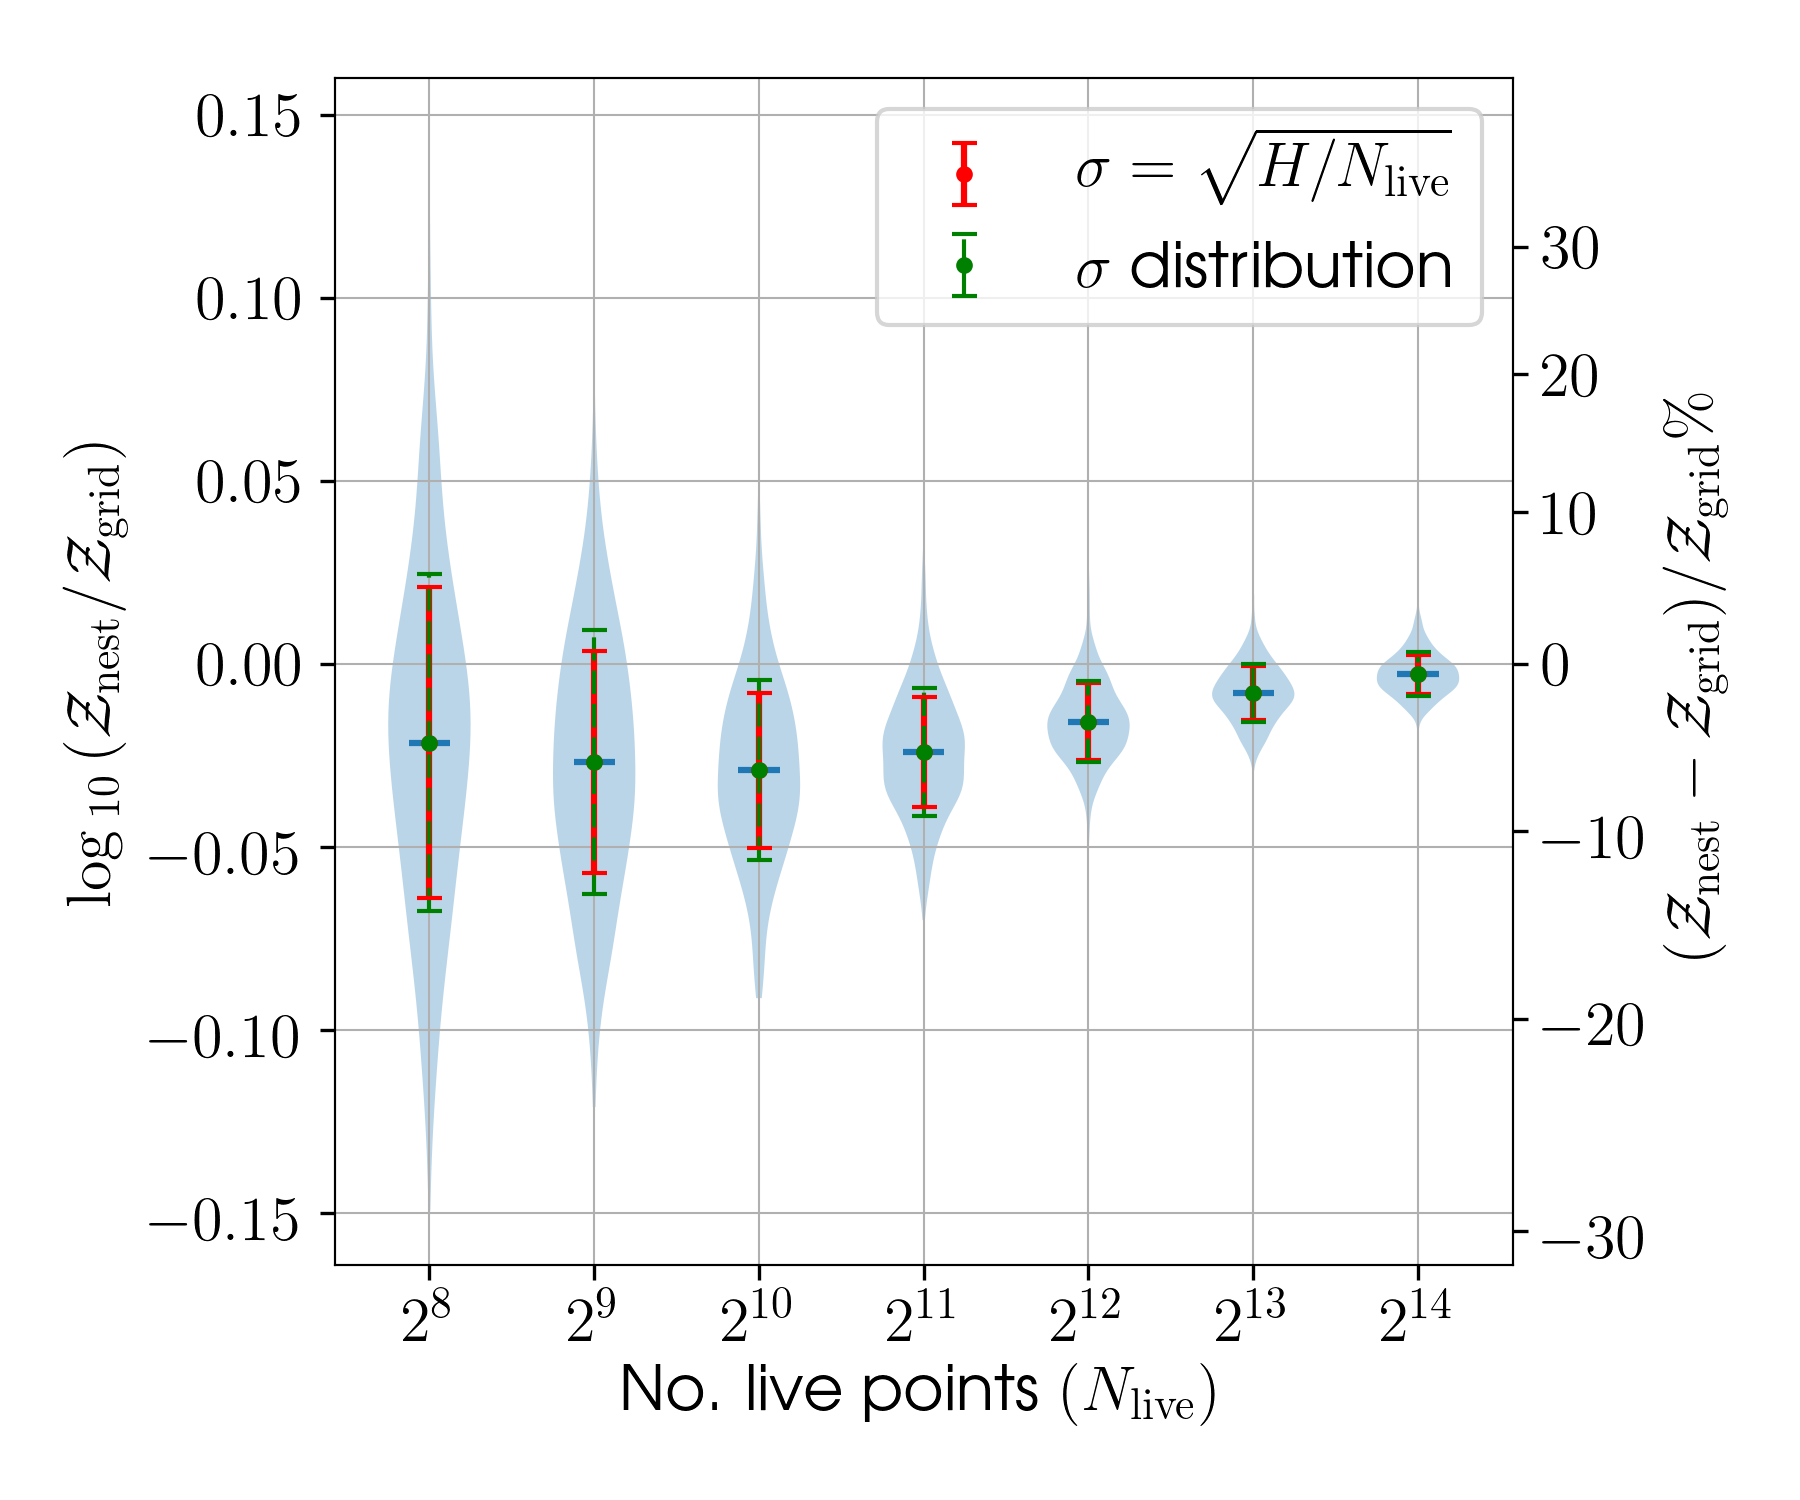
\includegraphics[width=1\columnwidth]{./figures/codeeval/stats/nest_evs/nest_evs}
\caption{ \protect\label{fig:nest_evs}
The distributions of ratios of evidence values calculated as a function of the number of live points used, based on searches over $h_0$, $\cos{\iota}$,
$\psi$ and $\phi0$ on 500 simulated Gaussian noise realisations for each $N_{\text{live}}$ value. The ratio compares the evidence produced by the
nested sampling algorithm in \lppen to that produced from a grid over the parameter space with \lppe (which we assume is a representation of the
true value). A comparison of the estimated error on the evidence value using the information gain, $H$ (which is $\sim 2.4$ here), with the measured
standard deviation of the distributions is also plotted and agree rather well.
}
\end{center}
\end{figure}

In Figure~\ref{fig:uls} we see a comparison between the 95\% upper limits on $h_0$ as a function of the number of live points. The core distribution of upper
limits produced via nested sampling are centred around the true (or grid-based) values, with the distribution decreasing with increasing numbers of live points.
The standard deviation on the distribution roughly follows $2^{6.8}N_{\text{live}}^{-1/2}$. The figure shows some extreme outliers in the distributions, but it
if found that these outliers occur in the cases when the number of posterior samples drawn from the nested samples is extremely low (the lower tails of the
distributions in Figure~\ref{fig:numposts}).

\begin{figure}[!phtb]
\begin{center}
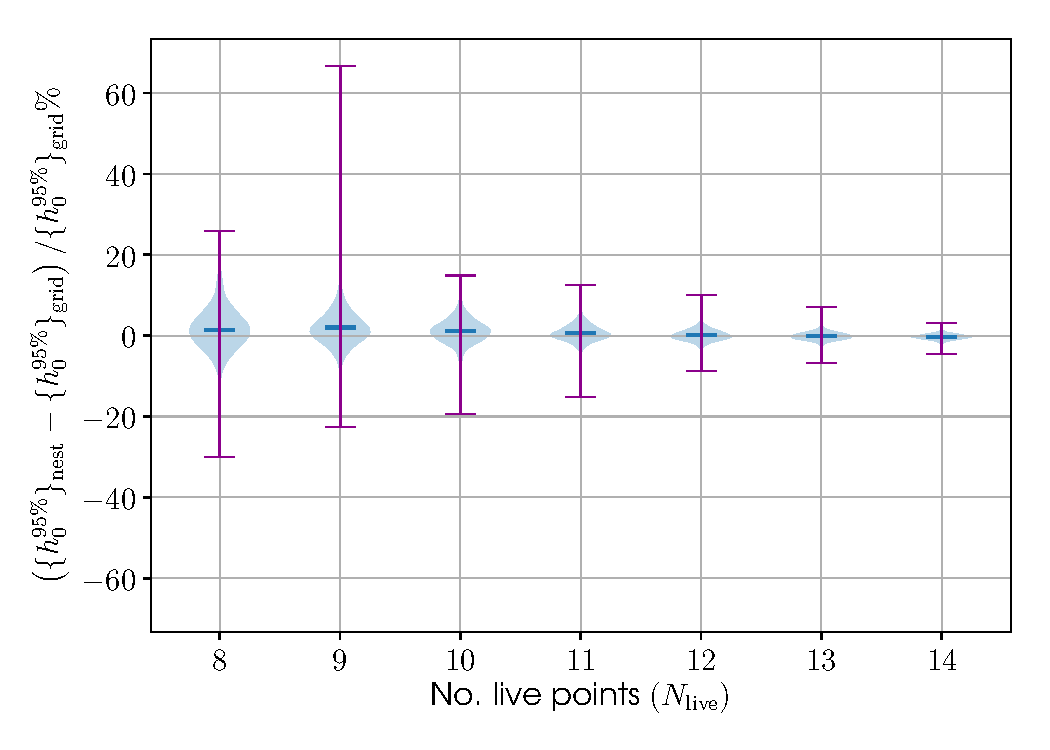
\includegraphics[width=1\columnwidth]{./figures/codeeval/stats/uls/uls}
\caption{ \protect\label{fig:uls}
The distribution of 95\% credible upper limits on $h_0$ as a function of number of live points
used.
}
\end{center}
\end{figure}

\subsection{Injections into real data}

During all bar the first initial LIGO science run, simulated signals from a variety of sources have been physically ``injected'' into the detector
datastreams. These are known as ``hardware injections'' \citep[see][for a general discussion of hardware injections, in particular relating to their
use, and extraction, in advanced LIGO's first obersving run]{2016arXiv161207864B}. These have included a range of continuous wave signals of the form given
by, e.g., Equation~2 of \citet{2017arXiv170107709T}, which in past have been searched for using a variety of analysis pipelines, including the one
described in this document using \lppe \citep[see, e.g., Appendix~B of][]{2007PhRvD..76d2001A}.

Here we have used \lppen to perform parameter estimation on the parameters $\vec{\theta} = \{h_0, \cos{\iota}, \psi, \phi_{0}\}$\footnote{$\phi_0$ is
being used here as opposed to $\Phi_{22}^C$ as we are not having to compare to the previous code.} for two hardware injections added to intial LIGO
data from the sixth science run (S6). These are two out of the thirteen total continuous wave injections and where called ``Pulsar03'' and ``Pulsar05''
respectively. The data have been heterodyned with the known phase evolution of the signals. The extracted posterior distributions can be seen in
Figures~\ref{fig:hwinj03} and \ref{fig:hwinj05} and are in very good agreement with the injection parameters.\footnote{For these hardware injections
exact agreement between the expected injection parameters and those recovered, or between detectors, is not entirely expected. This is due to the
injections needing to be performed using actuation functions (converting the expected \gw strain into a force required to be exerted in the
interferometer test mass) that may not exactly match the actuations functions later required for calibrating the detectors.} For ``Pulsar03''
the signal is recovered with SNRs of 164 and 96 in H1 and L1 respectively, and a coherent SNR of 190, and with
$\log{}_{10}\left(\mathcal{O}_{\text{S}/\text{N}}\right) = 6729$ and $\log{}_{10}\left(\mathcal{O}_{\text{S}/\text{I}}\right) = 9.1$. For ``Pulsar05''
the signal is recovered with SNRs of 9.9 amd 6.4 in H1 and L1 respectively, and a coherent SNR of 11.8, and with
$\log{}_{10}\left(\mathcal{O}_{\text{S}/\text{N}}\right) = 22.5$ and $\log{}_{10}\left(\mathcal{O}_{\text{S}/\text{I}}\right) = 4.6$.

\begin{figure}[!phtb]
\begin{center}
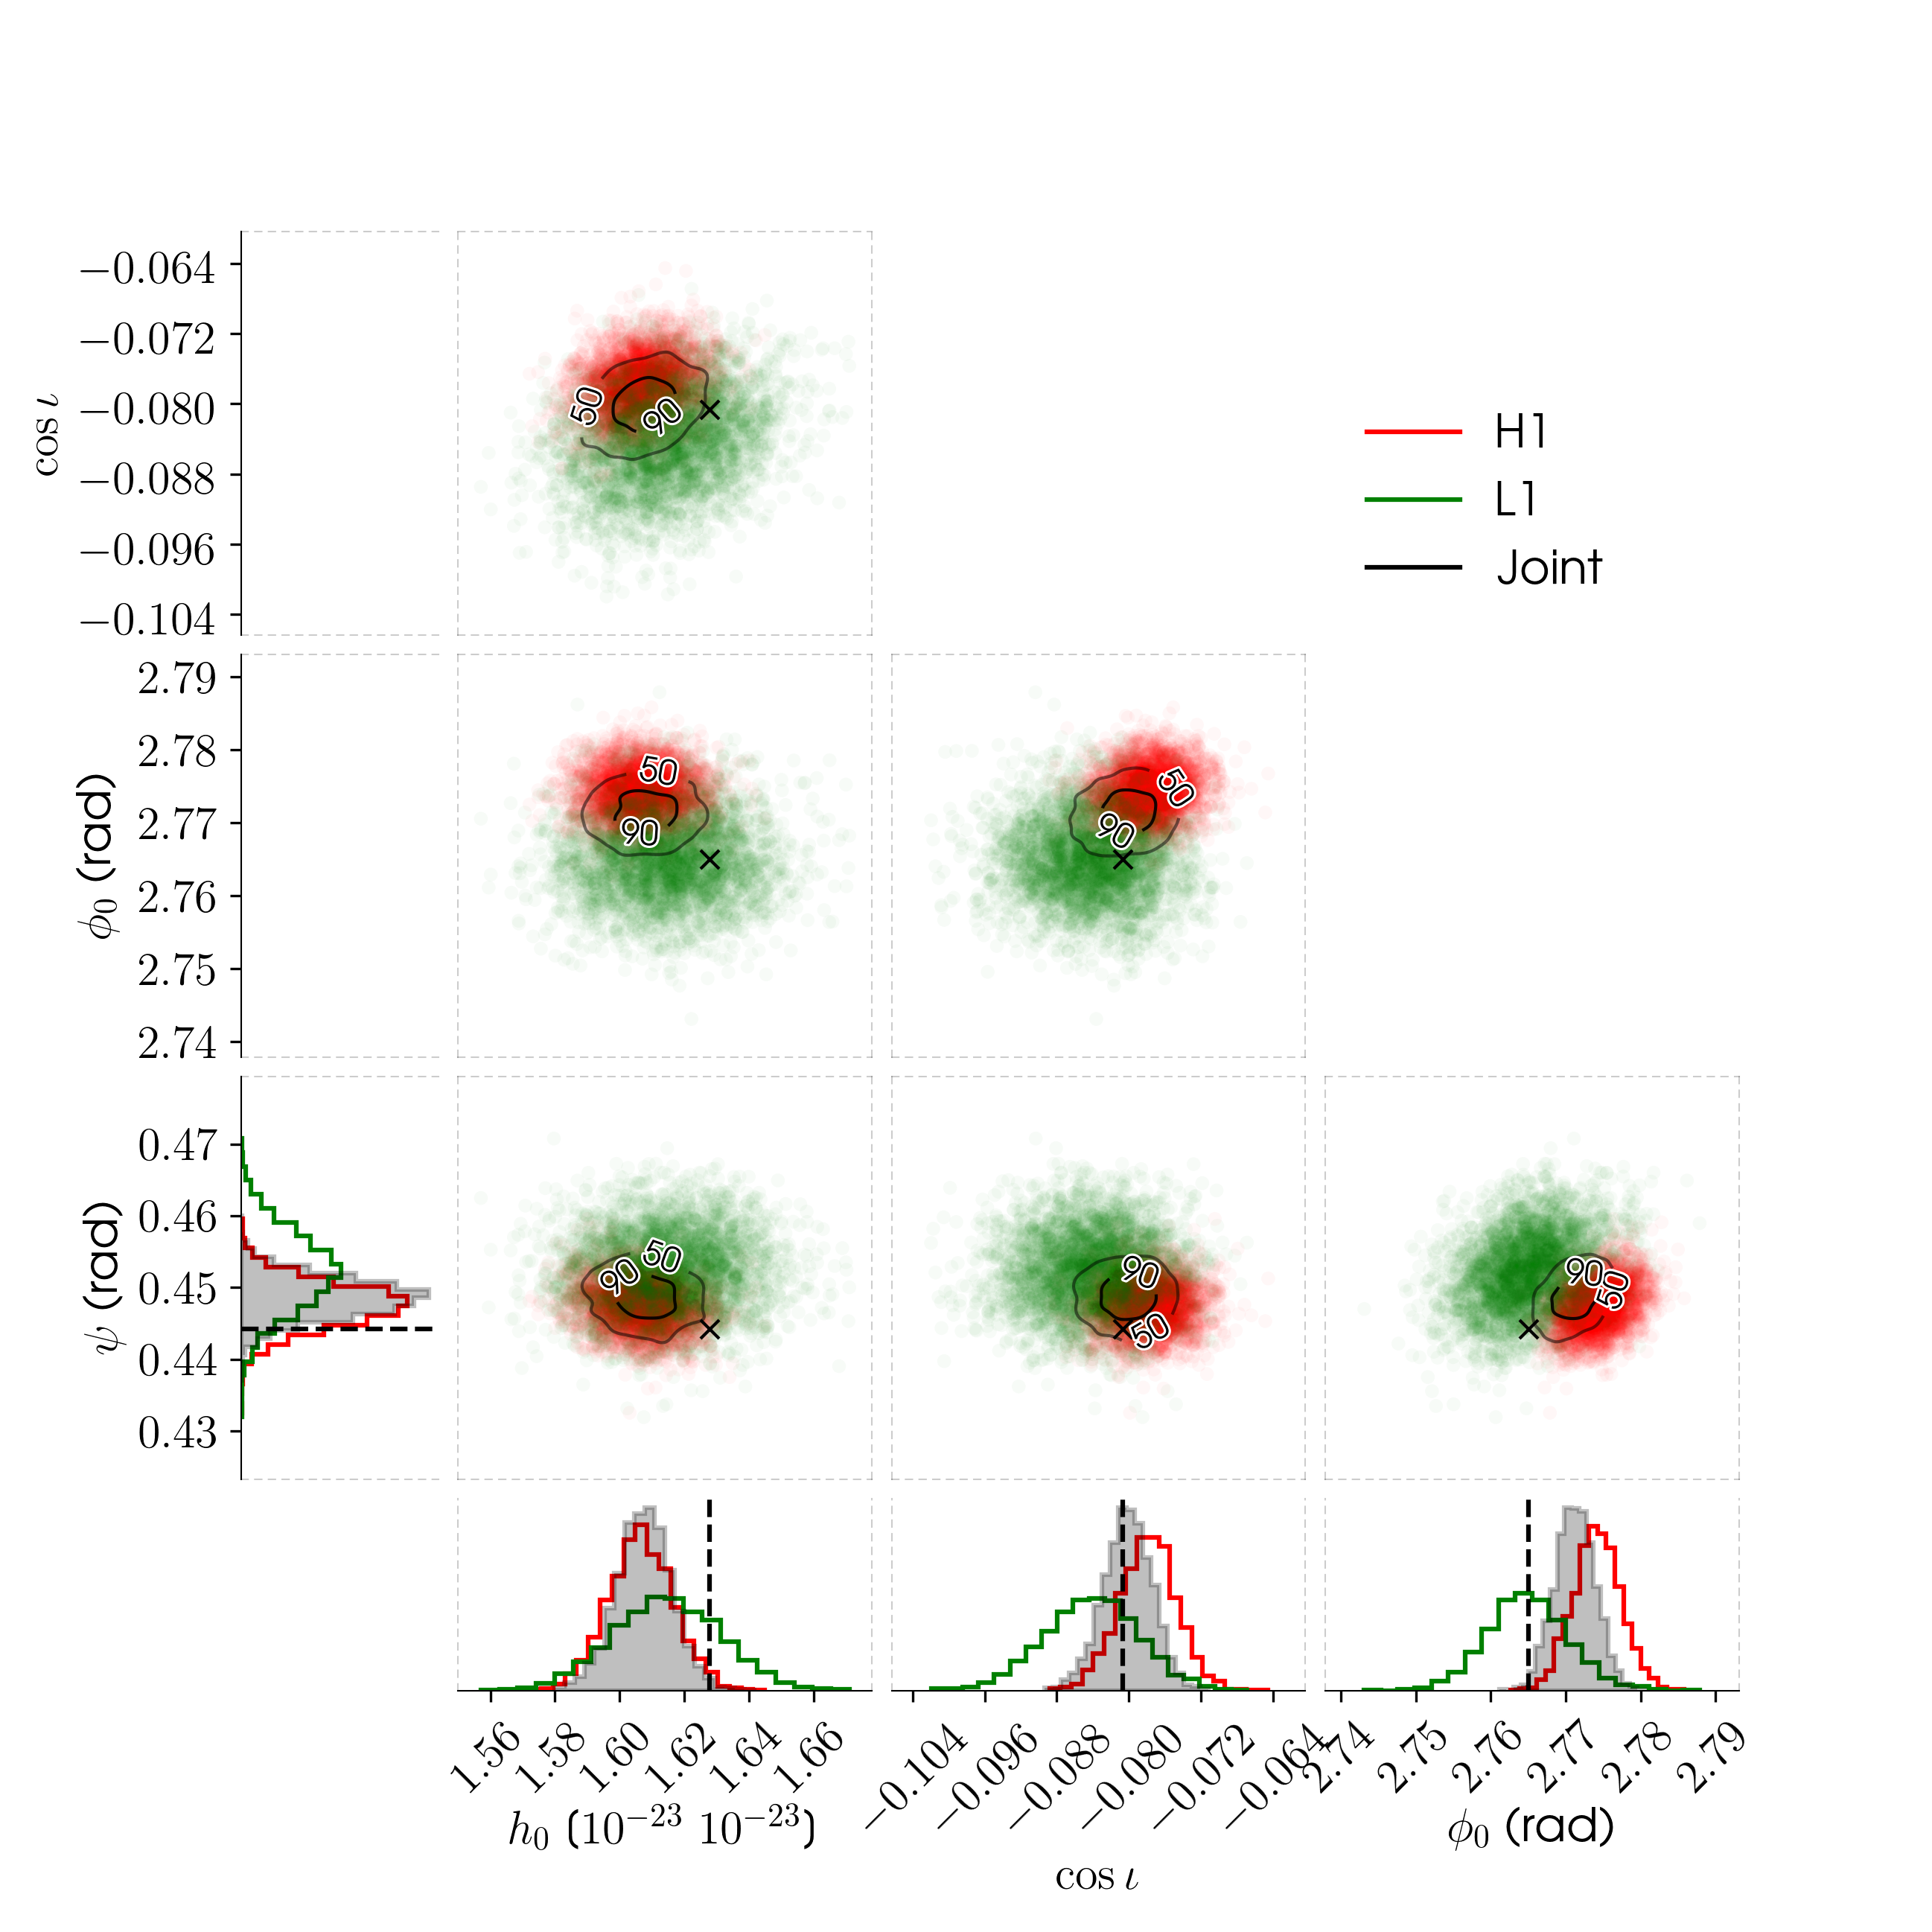
\includegraphics[width=1\columnwidth]{./figures/codeeval/simulations/S6_hwinj/hwinj03/hwinj03}
\caption{ \protect\label{fig:hwinj03}
Posterior probability distributions for the recovered parameters of a hardware injection (named ``Pulsar03'')
into LIGO sixth science run data. The black dashed lines and black crosses represent the expected signal
parameters.
}
\end{center}
\end{figure}


\begin{figure}[!phtb]
\begin{center}
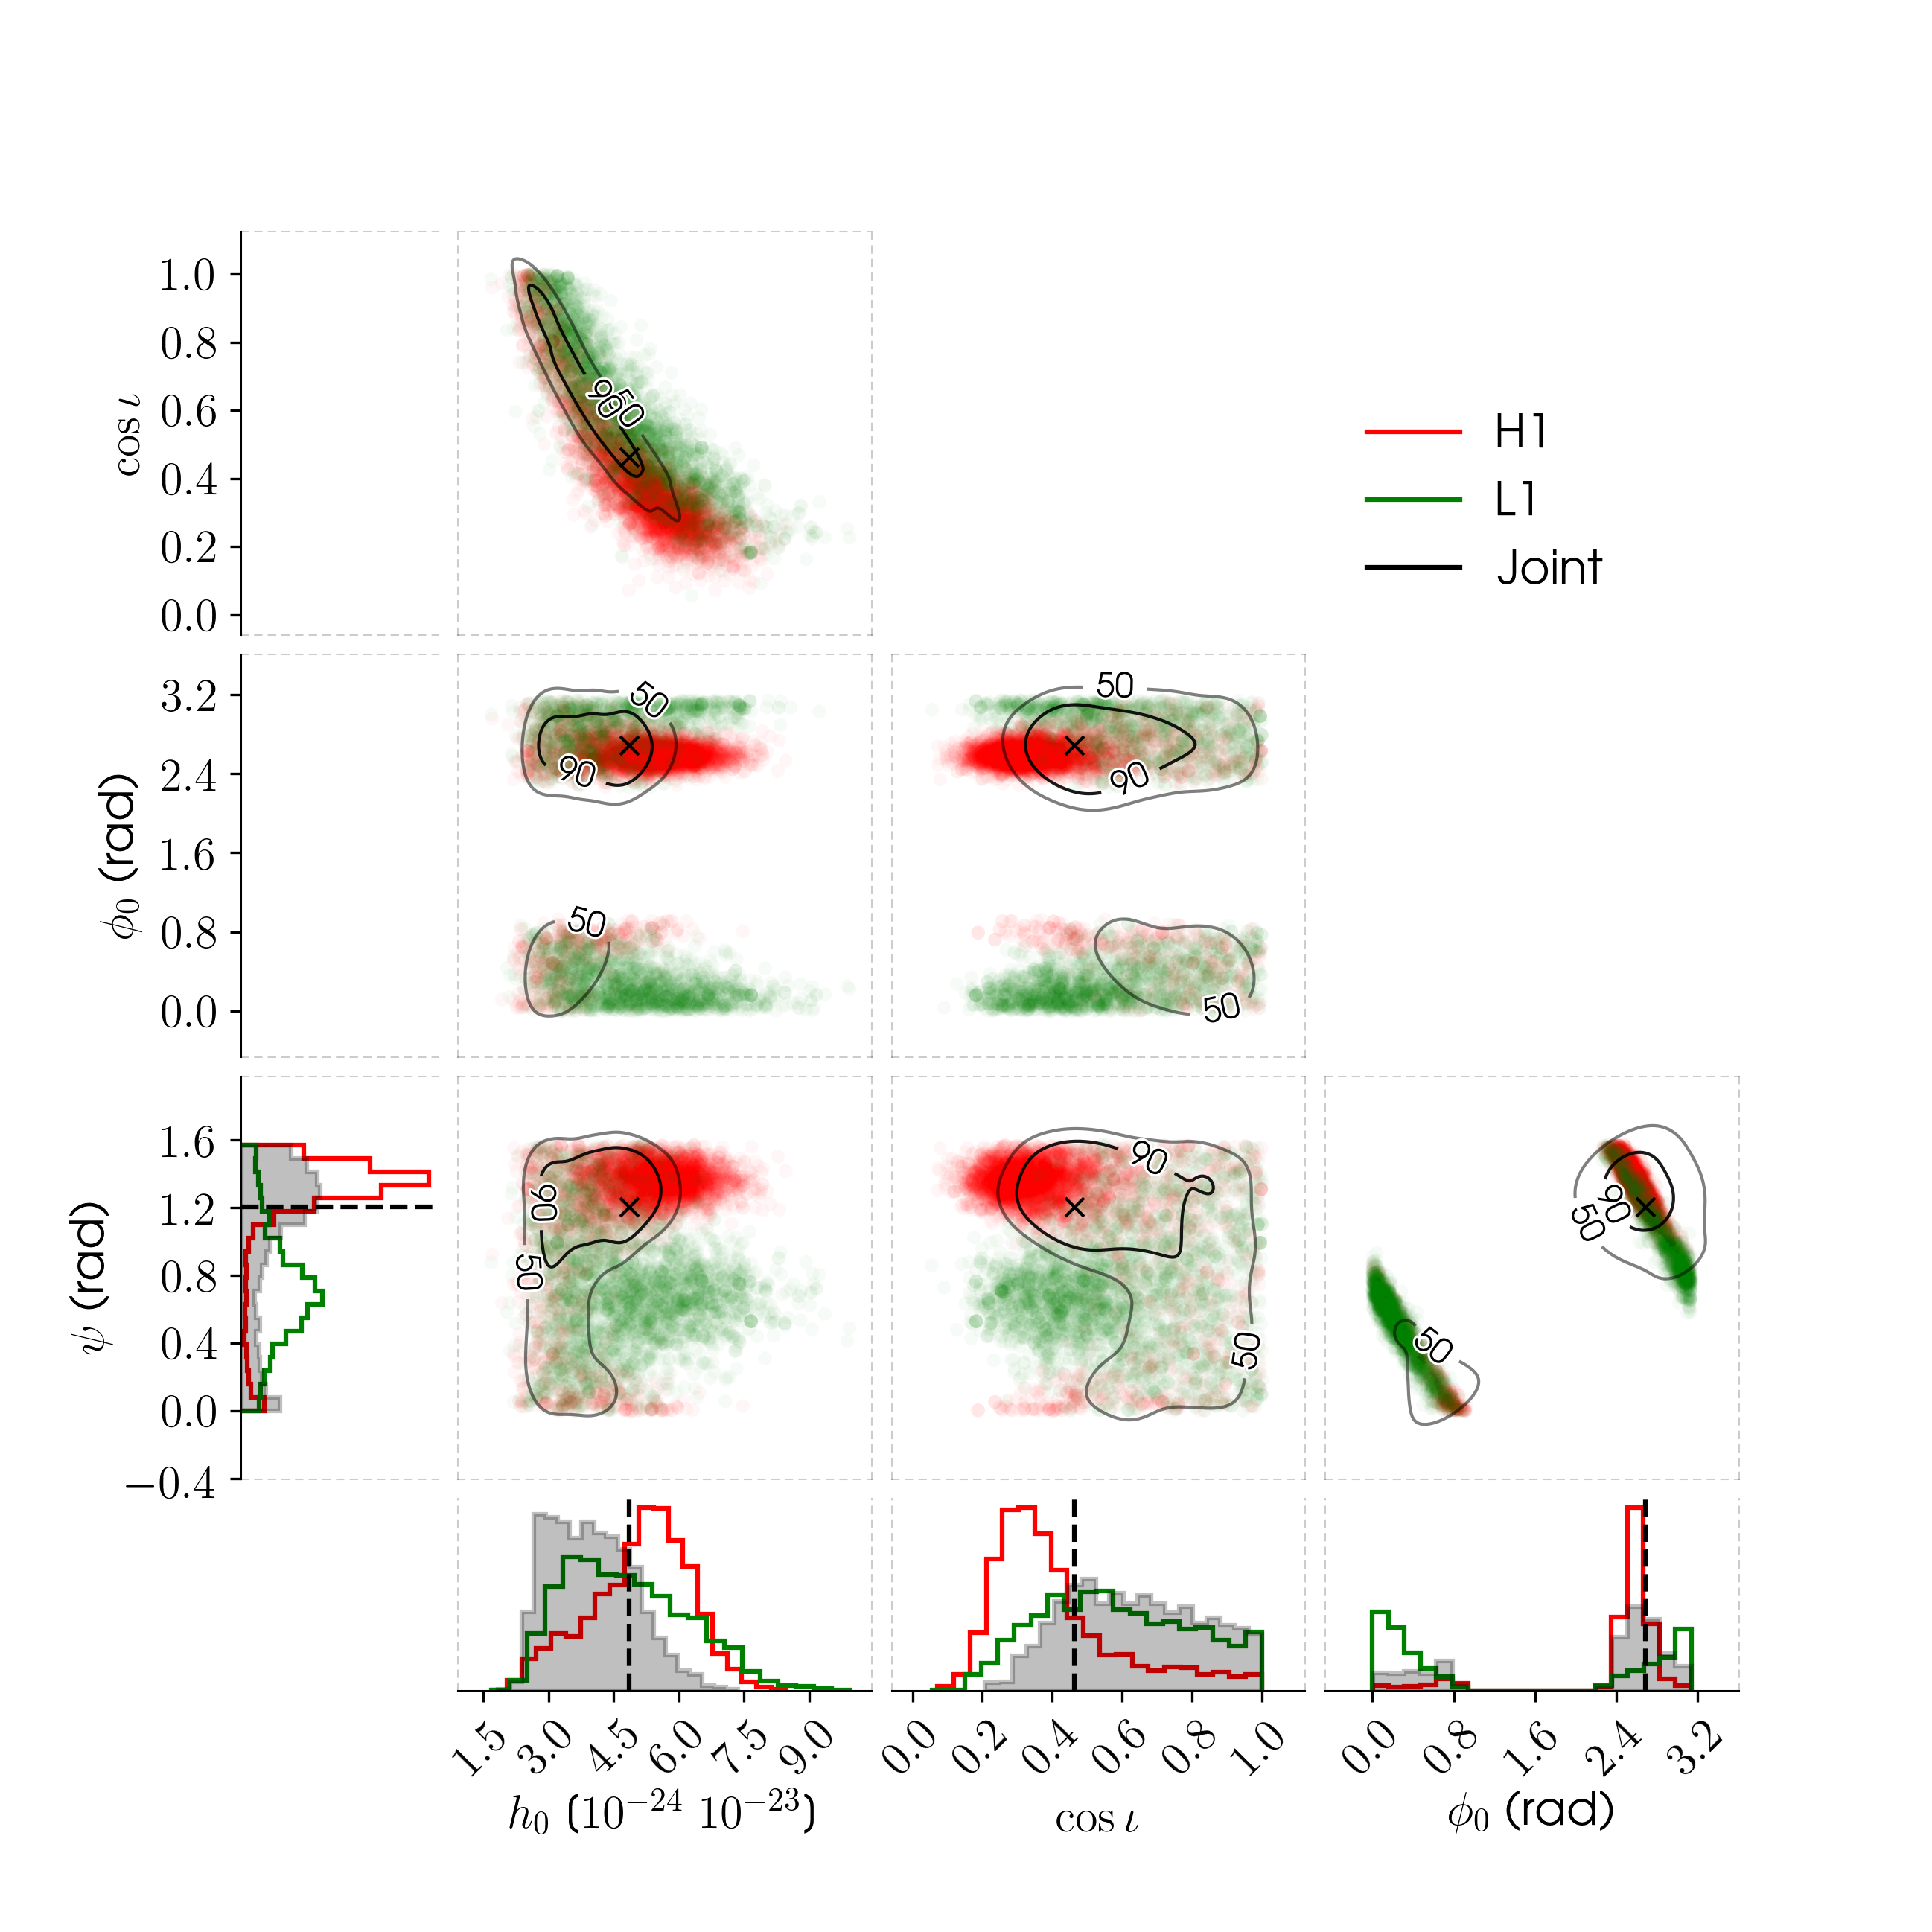
\includegraphics[width=1\columnwidth]{./figures/codeeval/simulations/S6_hwinj/hwinj05/hwinj05}
\caption{ \protect\label{fig:hwinj03}
Posterior probability distributions for the recovered parameters of a hardware injection (named ``Pulsar05'')
into LIGO sixth science run data. The black dashed lines and black crosses represent the expected signal
parameters. Note that the probability contours for the joint detector analysis, in particular for the $\phi_0$
versus $\psi$ plot, are broader than the true distributions due to the smoothing kernel not handling the
parameter degeneracy well.
}
\end{center}
\end{figure}

\subsection{Monte-Carlo studies}

In this section we will assess the outputs of \lppen using a range of simulated signals. We have created two sets of 2000 signal parameters with which to
inject simulated signals into Gaussian noise (with the same standard deviation of $1\ee{-22}$) for the H1 and L1 detectors. Both sets have been generated
with $\phi_0$, $\psi$ and $\cos{\iota}$ drawn from uniform distributions over their minimal allowed ranges \citep[Table~1 of][]{2015MNRAS.453.4399P},
but the first set
calculates $h_0$ such that the coherent SNR (Equation~\ref{eq:snr}) is drawn uniformly between 0 and 20; the second set draws the $h_0$ uniformly between
0 and $3.25\ee{-22}$, such that the maximum coherent SNR (given the known noise level) is $\sim 55$. This latter set is used to evaluate the posterior
distributions as described below in \S\ref{sec:ppplots}, whilst both sets are used to evaluate odds distributions. The source's sky locations are drawn
uniformly from over the sky-sphere. For these analyses each
simulated data set is one solar day long, consisting of 1440 complex data points (generated as if heterodyned at precisely the known source phase evolution)
sampled once per minute. This data has been used to estimate the four parameters $h_0$, $\cos{\iota}$, $\phi_0$ and $\psi$, with each being given
a flat prior: the angles and cosine of orientation angle over their minimal ranges, and $h_0$ between zero and $1\ee{-20}$ (well above the extent of the
bulk of the likelihood). When running \lppen on these, two parallel runs with 1024 live points where used, along with the default sampler proposals described
in \S\ref{sec:proposals}, and with the samples from both runs being combined to produce posterior samples and evidence estimates.

Another set of 2000 simulations has been created that again create simulated signals and add them to Gaussian noise for the H1 and L1 detectors. In this
case the total SNR shared between the detector has be drawn from a uniform distribution between 0 and 30, however, the signals have been purposely created
to be incoherent between detectors. The parameters $\phi_0$, $\psi$ and $\cos{\iota}$ are drawn from their minimal allowed ranges, but are different for
the signals input into the two detectors, whilst the sky positions are also independent for both detectors. The signal rotational frequency and frequency
derivative are also offset between detectors, such that the offsets are drawn from Gaussian distributions of $1/2048$\,Hz and $1\ee{-10}$\,Hz$\,s^{-1}$
respectively. The length of the data is the same as in the previous case, but it is assumed that the data for both detectors was heterodyned using the
known phase evolution for the signal in the just H1 detector. The same prior and run settings as above were used. These simulations have been used for
assessing the odds for a coherent versus incoherent signal (see \S\ref{sec:odds}).

Finally, two sets of simulations of 500 signals have been created to assess the code when estimating additional phase parameters: in this case
the rotational frequency $f_0$, frequency derivative $\dot{f}_0$, and right ascension $\alpha$. Gaussian priors on these three parameters have been
used, with parameters given in Table~\ref{tab:gaussianpriors}. These Gaussian priors are used when generating signals and when estimating them
using \lppen, whilst the simulated data is created such that it was heterodyned using the means values. As above, one set of these simulations has amplitude 
calculated such that the coherent SNRs are drawn uniformly between 0 and 20, whilst the other has amplitude drawn uniformly between 0 and $3.25\ee{-22}$.
The latter of these is used to evaluate the posterior distributions, whilst both are used for odds distributions assessment. Again, the angles are drawn
uniformly from their minimal ranges and sky positions are drawn uniformly over the sky-sphere.

\begin{table}[!hptb]
\caption{Gaussian prior parameters for rotational frequency, frequency derivative and right ascension for a set of simulated signals.
\label{tab:gaussianpriors}}
\begin{center}
\begin{tabular}{l | c c}
\hline
Parameter & mean & standard deviation \\                      
\hline
\hline
$f_0$ (Hz) & 100 & $5\ee{-5}$ \\
$\dot{f}_0$ & $-1\ee{-9}$ & $2\ee{-10}$ \\
$\alpha$ (rads) & $\pi$ & $0.0007272$ ($10^{\text{s}}$) \\
\hline
\end{tabular}
\end{center}
\end{table}

\subsubsection{Evaluating the posterior distributions}\label{sec:ppplots}

In \citet{2014PhRvD..89h4060S} a method was developed for evaluating whether sky location credible intervals for compact binary coalescence \gw signals, produced
from posterior distribution output by \lalinf codes \citep{2015PhRvD..91d2003V}, behaved self-consistently. The approach uses injected signal, with parameters
drawn from the prior distributions used when reconstructing them\footnote{In this case the amplitudes of the simulations are not drawn from the full prior range,
but are drawn from a flat distribution within that range, so are valid for this comparison.}, and sees if the credible intervals effectively behave as frequentist
confidence intervals, i.e.\ do 50\% of the known parameter values fall within some pre-specified definition (like the minimal credible region, or credible
region bounded by the lower extent to the prior) of the 50\% credible region. This can test whether the underlying \lalinf parameter sampling is working as
expected, or if there are biases to wider, or narrower, credible regions. The method, and the ``P-P plots'' it produces through evaluation over a range of credible
intervals, has now become commonly used to assess the \lalinf parameter estimation codes \citep{2015PhRvD..91d2003V} as a way of showing up any problems.

We have used this method here to evaluate our parameter posteriors produced from the simulations described above for which the amplitudes were drawn from
a uniform distribution. For each simulation we have calculated the minimal credible region from the one-dimensional marginalised posterior samples that the
injected value falls within (using a greedy-binning approach). The cumulative histogram of these values, for each parameter when using the simulations that
just estimate the four \gw parameters, can be seen in Figure~\ref{fig:pp_standard}. Also, shown for each parameter is a Kolmogorov-Smirnov test $p$-value
comparing our observed distribution to a uniform distribution, and a ``cloud'' of cumulative distributions that are random realisations of the expected
cumulative distribution. We see that, overall, our posteriors seem to produce posteriors that give credible intervals that behave as expected, without any
large deviations.

\begin{figure}[!phtb]
\begin{center}
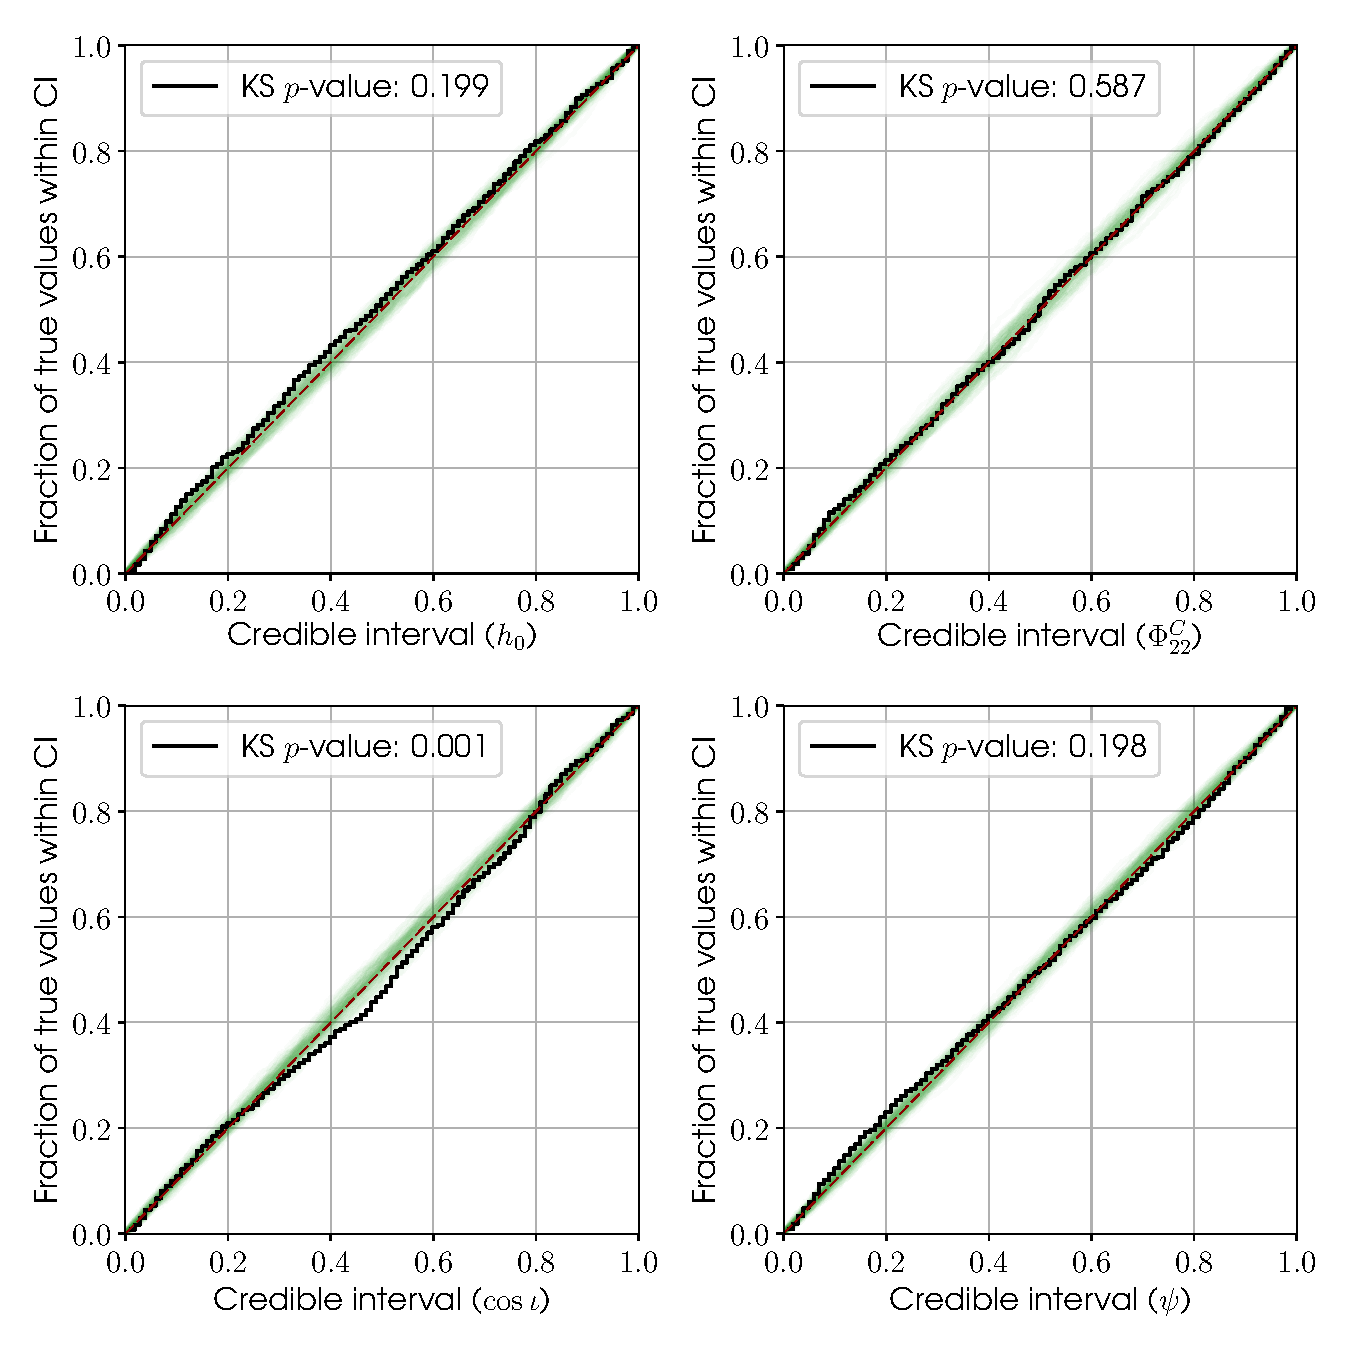
\includegraphics[width=1\columnwidth]{./figures/codeeval/stats/pp_standard/pp_plots_standard}
\caption{ \protect\label{fig:pp_standard}
The cumulative fraction of true parameter values (from simulated signals) found within
a particular credible interval.
}
\end{center}
\end{figure}

Similarly, we have done the same thing for the posteriors produced from the simulations that included searches over $f_0$, $\dot{f}_0$, and $\alpha$. 
In this case we know that the parameters are $f_0$ and $\phi_0$ are completely correlated (i.e.\ there is a degeneracy), so we have held the value of $\phi_0$
fixed at zero.\footnote{In cases where there is a degeneracy between parameters the samplers used in the code can have problems, leading to observable effects in
the ``P-P plots''. In certain cases, where the degeneracies are known, there are ways to deal with this: one parameter of a degenerate pair can be held fixed,
a custom proposal distribution can be hard coded for degenerate parameters that deals with the correlations, or, reparameterisations can be found that do not
have the degeneracies. In the future the latter of these may be implemented in our code to deal with strong degeneracies between the initial phase and derivatives of it
(frequency, and further frequency derivatives). Such a parameterisation could involve using, e.g.\ the start and end phase, rather than $\phi_0$ and $f_0$,
with further derivatives being incorporated through additional phase parameters at fixed times throughout the model. So, as another example, rather than
internally sampling in $\phi_0$, $f_0$, and $\dot{f}_0$, one could use $\phi_{\text{start}}$, $\phi_{\text{mid}}$, and $\phi_{\text{end}}$, and convert between
the two using linear algebra.} These ``P-P plots'' can be seen in Figure~\ref{fig:pp_extra}, where generally we see posterior credible intervals behaving as
expected.

\begin{figure}[!phtb]
\begin{center}
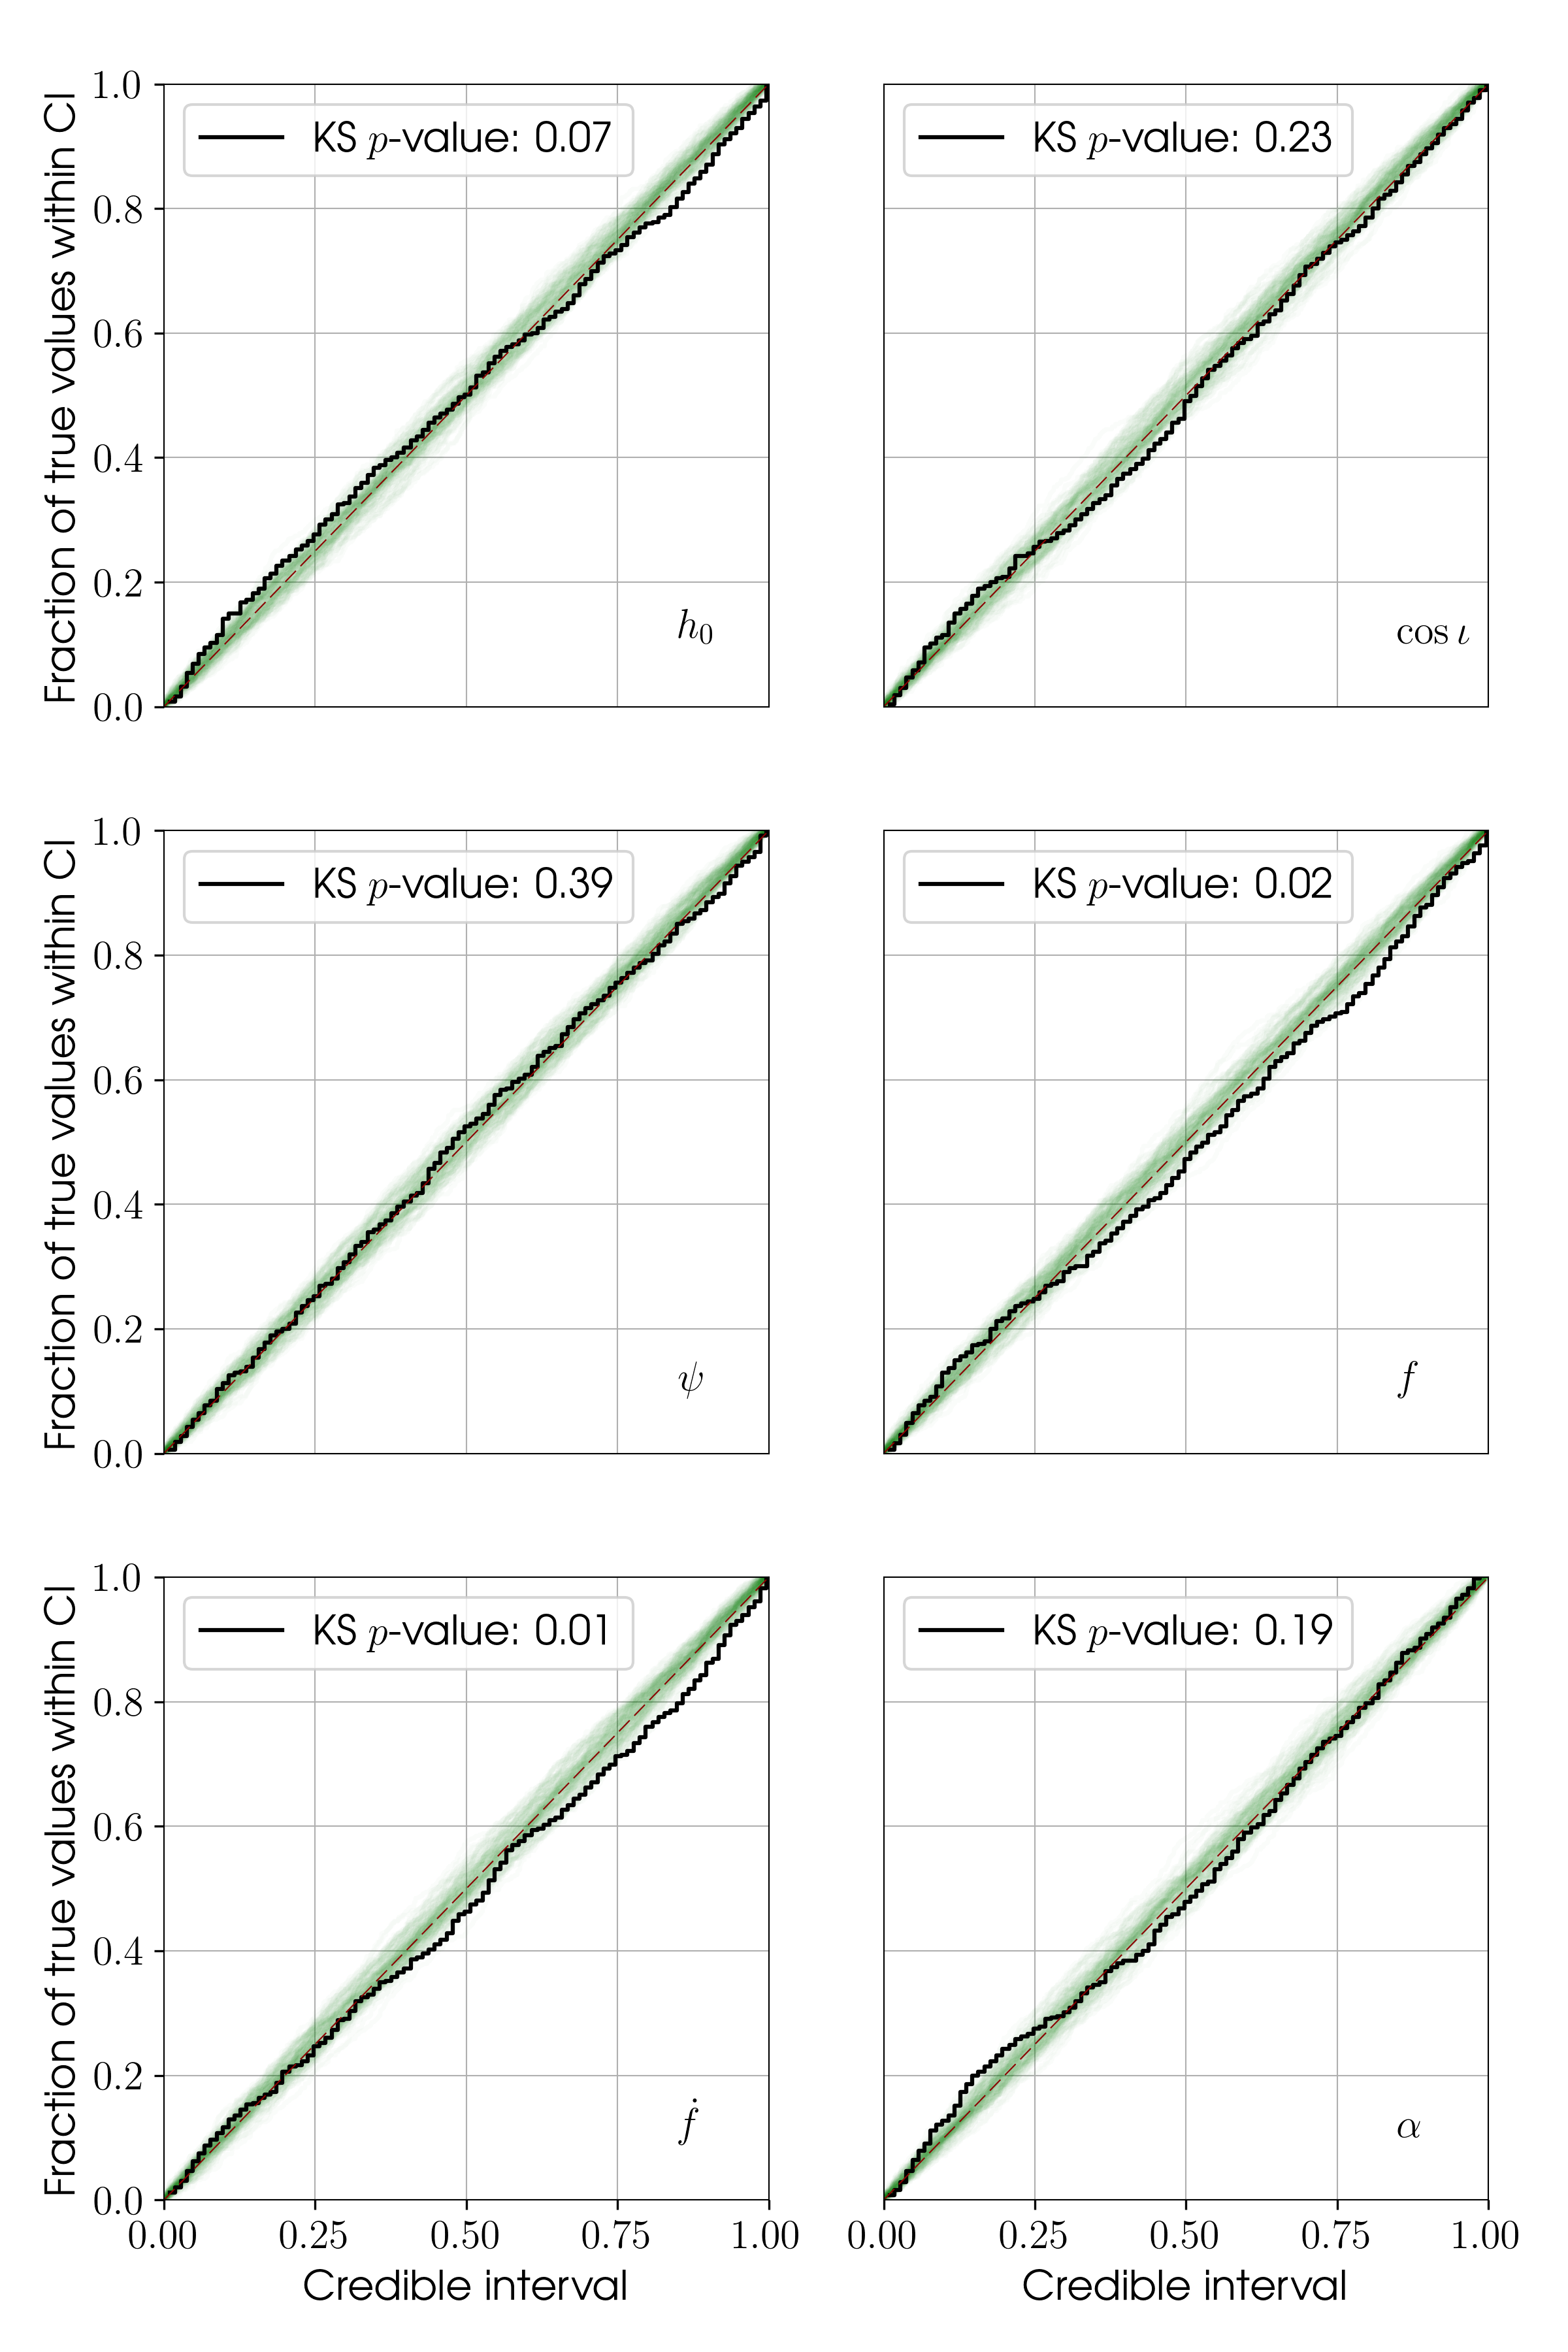
\includegraphics[width=1\columnwidth]{./figures/codeeval/stats/pp_extra/pp_plots_extra}
\caption{ \protect\label{fig:pp_extra}
The cumulative fraction of true parameter values (from simulated signals) found within
a particular credible interval.
}
\end{center}
\end{figure}

\subsubsection{Evaluating the odds}\label{sec:evalodds}

It is useful to see how the odds values, described in \S\ref{sec:odds}, look when calculated for our simulations. As mentioned above, along with coherent
signals between two detectors, we have purposely created incoherent signals to see how the odds look. Firstly, just considering the coherent simulations,
we can see in Figure~\ref{fig:snrvsodds} how the odds $\mathcal{O}_{\text{S}/\text{N}}$, $\mathcal{O}_{\text{S}/\text{I}}$ and
$\mathcal{O}_{\text{S}/\text{I}_{\text{simple}}}$ (Equations~\ref{eq:sigvsnoise}, \ref{eq:cohvincoh2} and \ref{eq:cohvincoh1}, respectively) vary as a function
of coherent SNR. We see that $\mathcal{O}_{\text{S}/\text{N}}$ rapidly increases, $\mathcal{O}_{\text{S}/\text{I}_{\text{simple}}}$ has a shallow growth,
whilst $\mathcal{O}_{\text{S}/\text{I}}$ transitions between following $\mathcal{O}_{\text{S}/\text{N}}$ at very low SNR to matching 
$\mathcal{O}_{\text{S}/\text{I}_{\text{simple}}}$ at higher SNR. This behaviour is consistent with our expectations described in Appendix~\ref{app:oddratios} with
$\ln{\mathcal{O}_{\text{S}/\text{N}}} \propto \rho_{\text{coh}}^2$ and $\mathcal{O}_{\text{S}/\text{I}_{\text{simple}}} \propto \rho_{\text{coh}}$.
We note that the locations of these distributions on the y-axis can be strongly effected by the prior volume, changes to which will move the distributions
up or down, and can affect where they intersect. However, the general shape of the distributions should be very similar.

\begin{figure}[!phtb]
\begin{center}
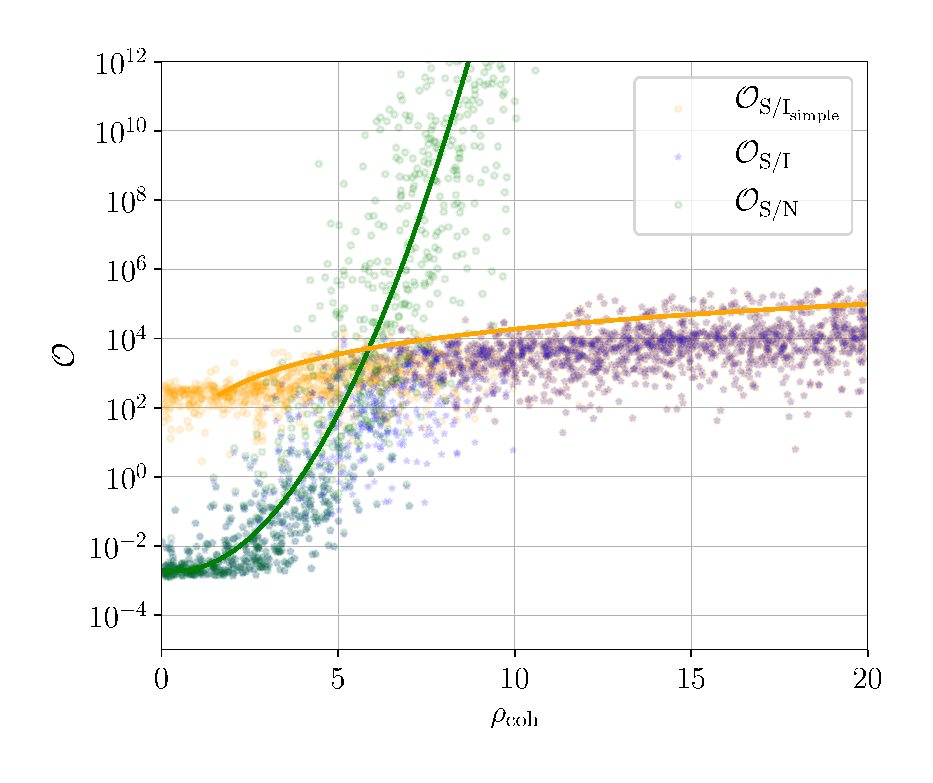
\includegraphics[width=1\columnwidth]{./figures/codeeval/stats/snr_vs_odds/snr_v_odds_plot}
\caption{ \protect\label{fig:snrvsodds}
Various odds values plotted as a function of the injected coherent signal-to-noise ratio ($\rho_{\text coh}$).
Shown are the (simple) coherent signal versus incoherent signal odds ($\mathcal{O}_{{\rm S/I}_{\rm simple}}$ given
in Equation~\ref{eq:cohvincoh1}), more complete coherent signal versus incoherent signal {\it or} noise odds
($\mathcal{O}_{\rm S/I}$ given in Equation~\ref{eq:cohvincoh2}), and coherent signal versus Gaussian noise odds
($\mathcal{O}_{\rm S/N}$ given in Equation~\ref{eq:sigvsnoise}). Also shown are lines with a quadratic fit
to the $\mathcal{O}_{\rm S/N}$ values, to show the $\log{\mathcal{O}_{\rm S/N}} \propto \rho_{\text{coh}}^2$ relation,
and a fit to show the $\mathcal{O}_{{\rm S/I}_{\rm simple}} \propto \rho_{\text{coh}}$ relation.
}
\end{center}
\end{figure}

In Figure~\ref{fig:oddsplot} there are two panels showing $\mathcal{O}_{\text{S}/\text{I}}$ as a function of $\mathcal{O}_{\text{S}/\text{N}}$. In the upper
panel a hexagon-binned histogram has been used to plot the distribution for the coherent injections, with the bin colours showing the average
coherent SNR. The plateauing of $\mathcal{O}_{\text{S}/\text{I}}$ is just that seen in Figure~\ref{fig:snrvsodds}. The bottom panel show the coherent signals
as red circles, with the incoherent signals as dark circles (these are also seen in the lower left of the upper panel). Here we see that for incoherent signals
the value of $\mathcal{O}_{\text{S}/\text{I}}$ between the coherent and incoherent signals diverges quite quickly, with $\ln{\mathcal{O}_{\text{S}/\text{I}}}$
falling off roughly linearly with $\mathcal{O}_{\text{S}/\text{N}}$. This shows that, hopefully, for reasonable strength signals the value of
$\mathcal{O}_{\text{S}/\text{I}}$ will be useful for distinguishing a coherent from an incoherent (and therefore not astrophyical) signal.\footnote{The caveats
to this are that the way we created our incoherent signals may not well match true signals caused by instrumental (non-astrophysical) effects in \gw detectors.
However, we hope our simulations are extreme, in a conservative way, in that one detector is actually containing an unadulterated signal, and is therefore
potentially producing a far larger $\mathcal{O}_{\text{S}/\text{N}}$ value than might be expected.}

\begin{figure*}[phtb]
\begin{center}
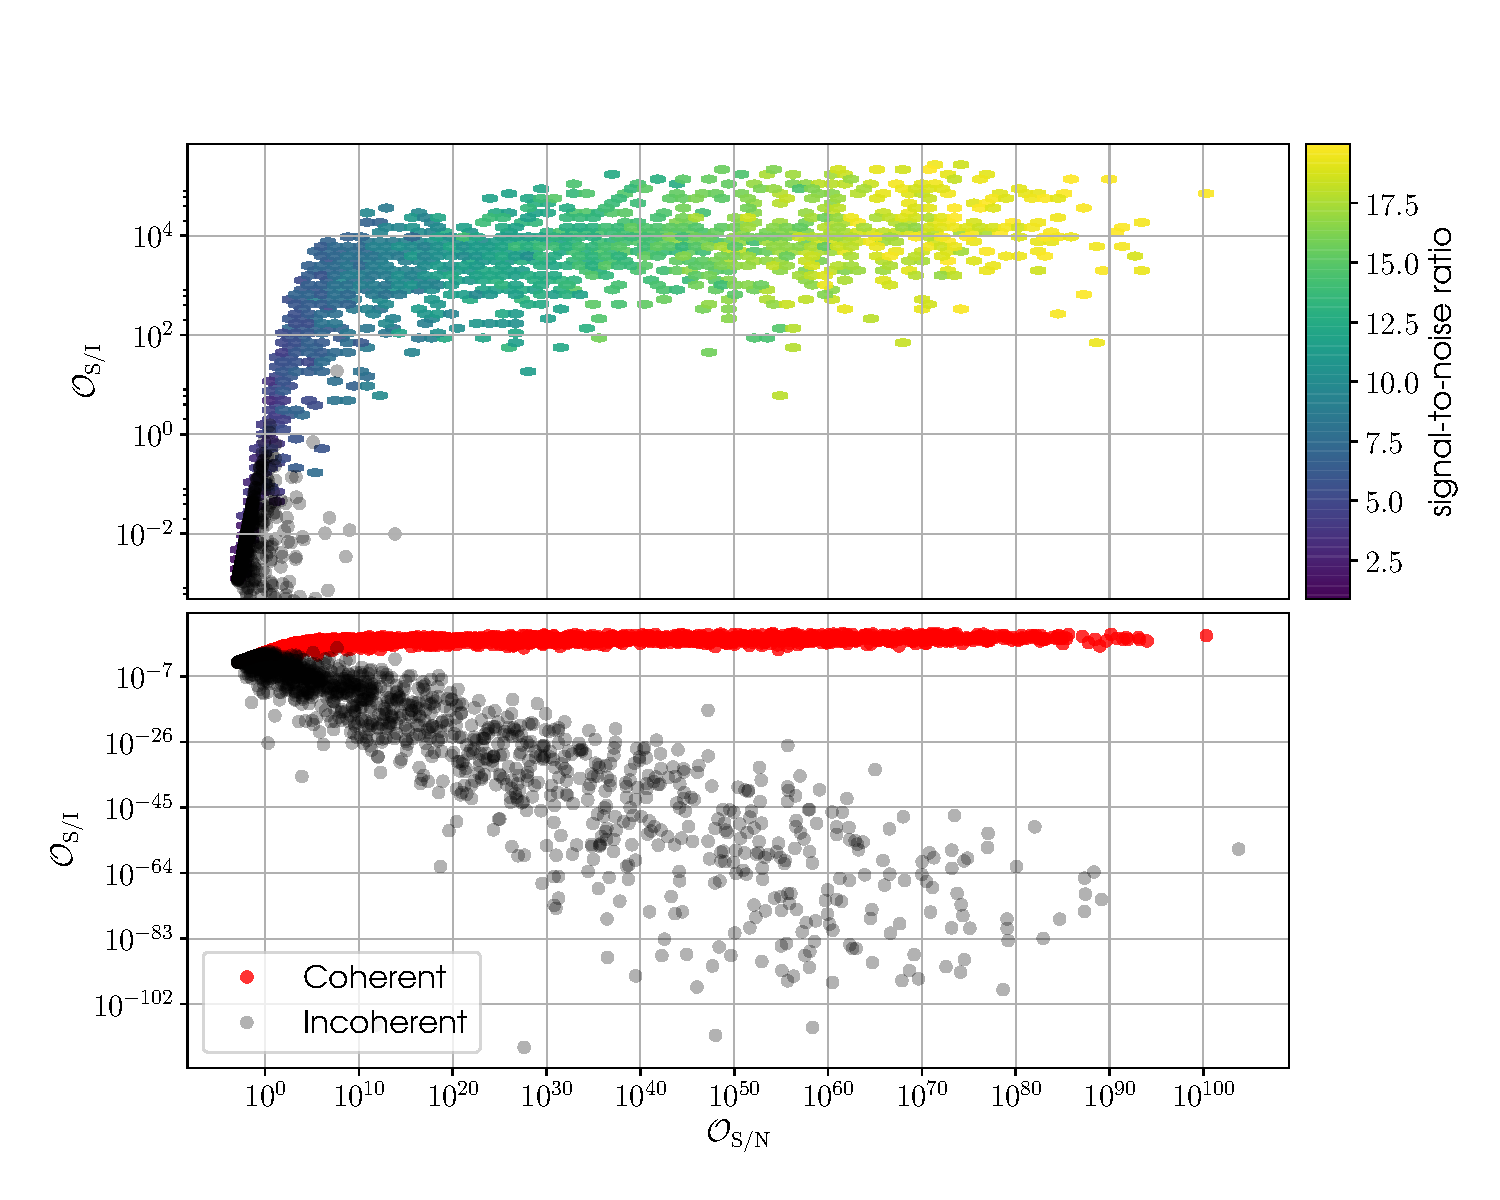
\includegraphics[width=0.7\textwidth]{./figures/codeeval/stats/odds/odds_plot}
\caption{ \protect\label{fig:oddsplot}
The coherent signal versus incoherent signal {\it or} noise odds ($\mathcal{O}_{{\rm S/I}_{\rm simple}}$ given
in Equation~\ref{eq:cohvincoh2}) plotted against the coherent signal versus noise odds ($\mathcal{O}_{\rm S/N}$ given
in Equation~\ref{eq:sigvsnoise}), for simulated signals injected as if into the two LIGO Hanford and Livingston
detectors. Half the simulations were created with coherent signals between the two detectors (hexagonal-binned histogram
points in the upper plots, and red points in the lower plot), whilst the other half where incoherent between the
two detectors (black points in both plots). The upper plot is a zoomed in version of the lower plot, with hexagonal
histogram bins coloured to show the coherent signal SNR.
}
\end{center}
\end{figure*}

The above simulations were all performed with signal searches over only $h_0$, $\cos{\iota}$, $\phi_0$ and $\psi$. Uncertainties on other parameter will
likely cause things to change, but it is expected that the distributions would look broadly similar with the main changes being slight rescalings of the axes.

It is useful to see how these distributions change when the parameter space searched over increases in complexity. So, in Figure~\ref{fig:snrvsodds_larger}
we see similar plots to those above, but for the simulations that included searches over $f_0$, $\dot{f}$, and $\alpha$ (but fixed $\phi_0$). In the left
panel we see $\mathcal{O}_{\text{S}/\text{N}}$ and $\mathcal{O}_{\text{S}/\text{I}}$ as a function of $\rho_{\text{coh}}$ for these simulations, with the
earlier simulations plotted underneath. It is obvious that for these injections that these odds follow the same form as before, however, at low SNR there
is more scatter in $\mathcal{O}_{\text{S}/\text{I}}$ than seen before. This can be interpreted as finding spikes in $f_0\operatorname{-}\dot{f}$-space, that
are not related to the signal, in individual detectors, which are therefore not coherent. For higher SNRs ($\gtrsim 10$) the $\mathcal{O}_{\text{S}/\text{I}}$
value for
this more complex search does tend to give higher values than for the simpler search. A hand-wavy explanation for this could be that a truely coherent signal
found (at large enough SNR) within this larger space is more convincing (more parameters have to match up) than in the simpler case, and this outweights any
prior Occam factor. The right panel of Figure~\ref{fig:snrvsodds_larger} shows similar information.

\begin{figure*}[phtb]
\begin{center}
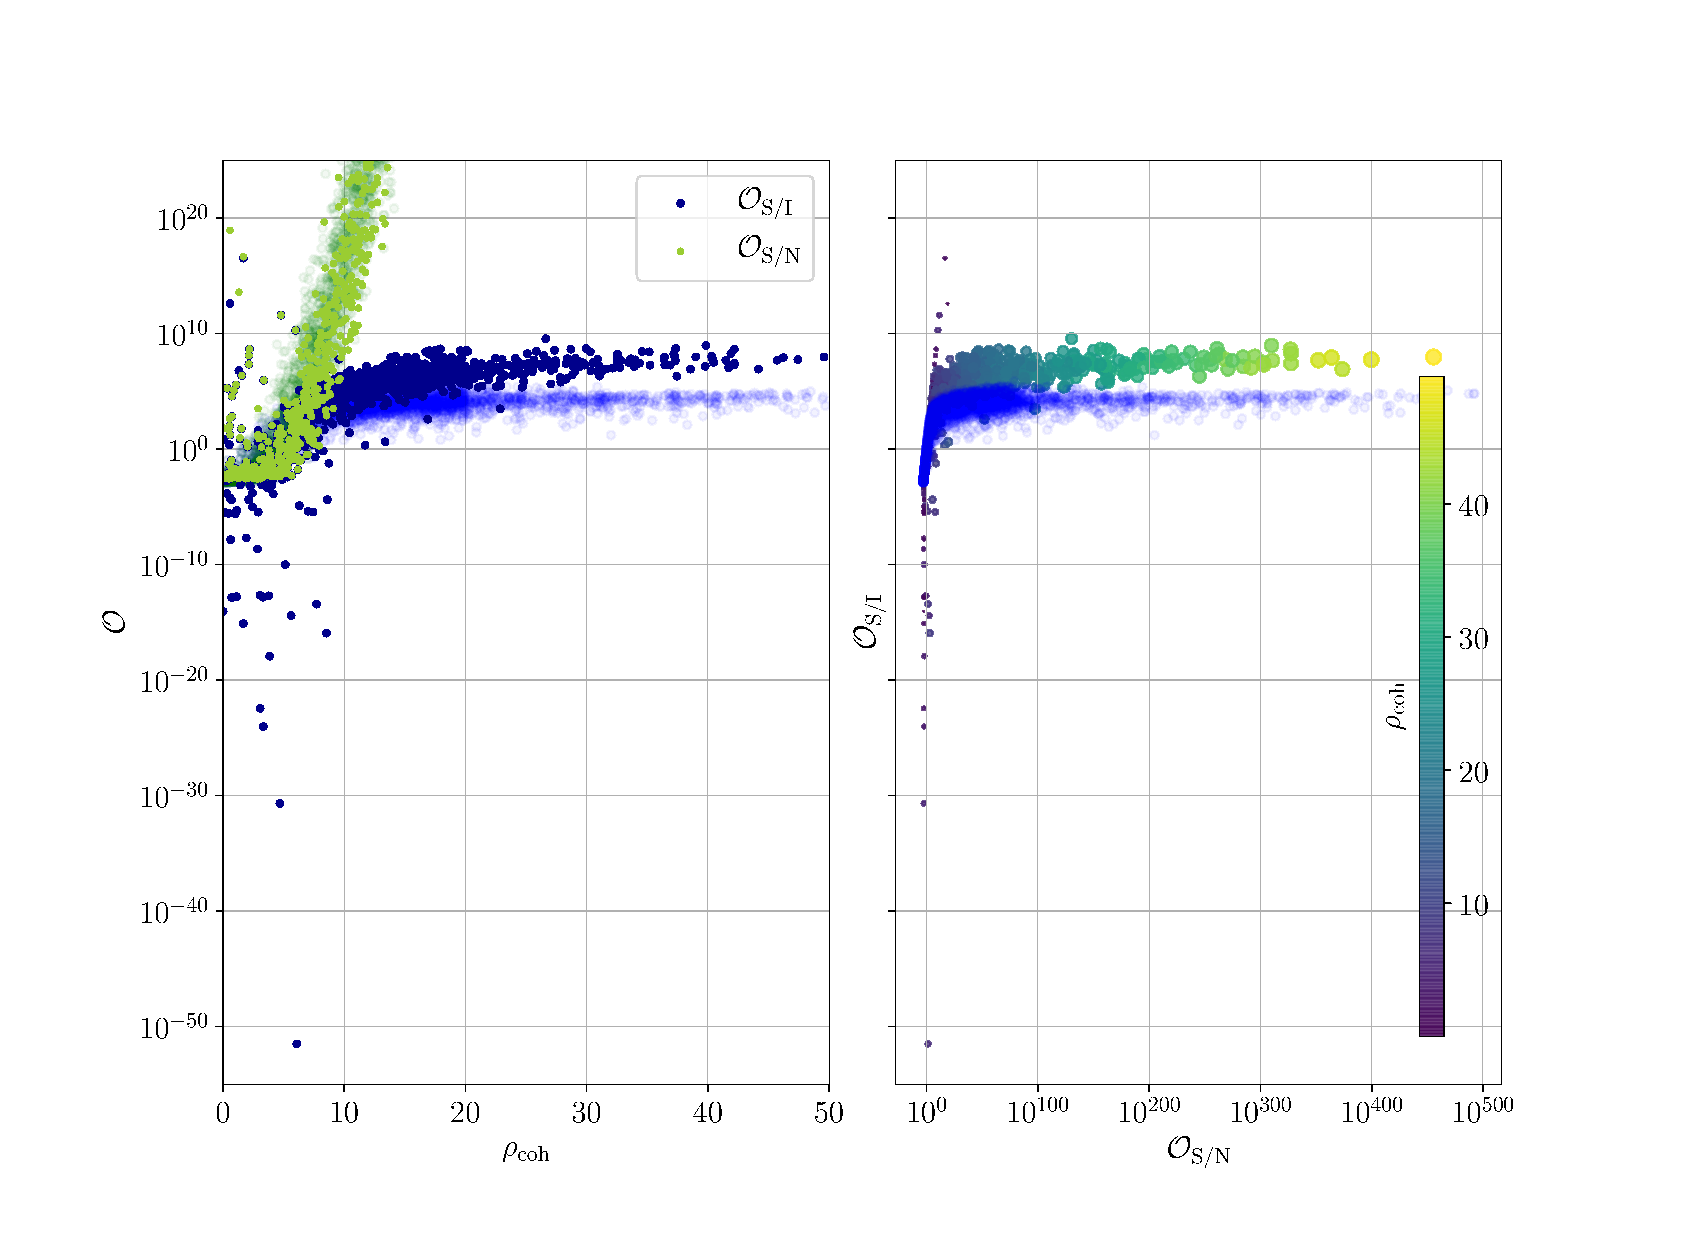
\includegraphics[width=0.8\textwidth]{./figures/codeeval/stats/snr_vs_odds_larger/snr_v_odds_larger_plot}
\caption{ \protect\label{fig:snrvsodds_larger}
Plots showing odds values for a range of simulated signals for searches over the seven parameters of $h_0$, $\phi_0$,
$\cos{\iota}$, $\psi$, $f_0$, $\dot{f}$, and $\alpha$. The solid points in the left panel shows two odds values
($\mathcal{O}_{\rm S/I}$ and $\mathcal{O}_{\rm S/N}$) plotted as a function of the injected coherent signal-to-noise ratio
($\rho_{\text coh}$). Also shown, underplotted as shaded circles, are the value for the four parameter search seen in
Figure~\ref{fig:snrvsodds}. The right plot shows $\mathcal{O}_{\rm S/I}$ as a function of $\mathcal{O}_{\rm S/N}$, with
the colour of each point giving the coherent SNR. Also shown, as the light blue circles, are the values for the four
parameter search seen in Figure~\ref{fig:oddsplot}.
}
\end{center}
\end{figure*}

\subsubsection{Further parameter estimation}

In Figures~\ref{fig:ffdot_inj1} and \ref{fig:ffdot_inj1} we show the posterior distributions for two of the simulations performed for the searches over
$h_0$, $\cos{\iota}$, $\phi_0$, $\psi$, $f_0$, $\dot{f}$, and $\alpha$ above.\footnote{Earlier, during the discussing of the ``P-P plots'' in \S\ref{sec:ppplots},
it was mentioning that $\phi_0$ was held fixed due to the degeracies between $f_0$ and $\phi_0$. In this case, as we also have $\dot{f}$ the correlations
become more complex, and whilst it would be expected that holding $\phi_0$ fixed would give valid posteriors, it is in such cases that a re-parameterisation
may be more appropriate.} The simulation in Figure~\ref{fig:ffdot_inj1} had injected SNRs of 4.4 and 6.5 for H1
and L1 respectively, with a coherent SNR of 7.9, and the recovered values of $\log{}_{10}\mathcal{O}_{\text{S}/\text{N}}$ and
$\log{}_{10}\mathcal{O}_{\text{S}/\text{I}}$ of 1.55 and 0.95 respectively. It can be seen that the search in H1 alone finds additional structure
in the frequency space, whilst in L1 the signal dominates, and the joint analysis also recovers the signal. The simulation in Figure~\ref{fig:ffdot_inj2}
is a little stronger with injected SNRs of 7.3 and 8.5 for H1 and L1 respectively, and a coherent SNR of 11.2, and recovered values of 
$\log{}_{10}\mathcal{O}_{\text{S}/\text{N}}$ and $\log{}_{10}\mathcal{O}_{\text{S}/\text{I}}$ of 23.8 and 6.3 respectively. The signal is by far the strongest
feature in the data, and not other structure is present in the posteriors. The first signal would probably only rate as marginal if determining whether it was
a true signal or not, whereas the second signal would be a clear detection.

\begin{figure}[!phtb]
\begin{center}
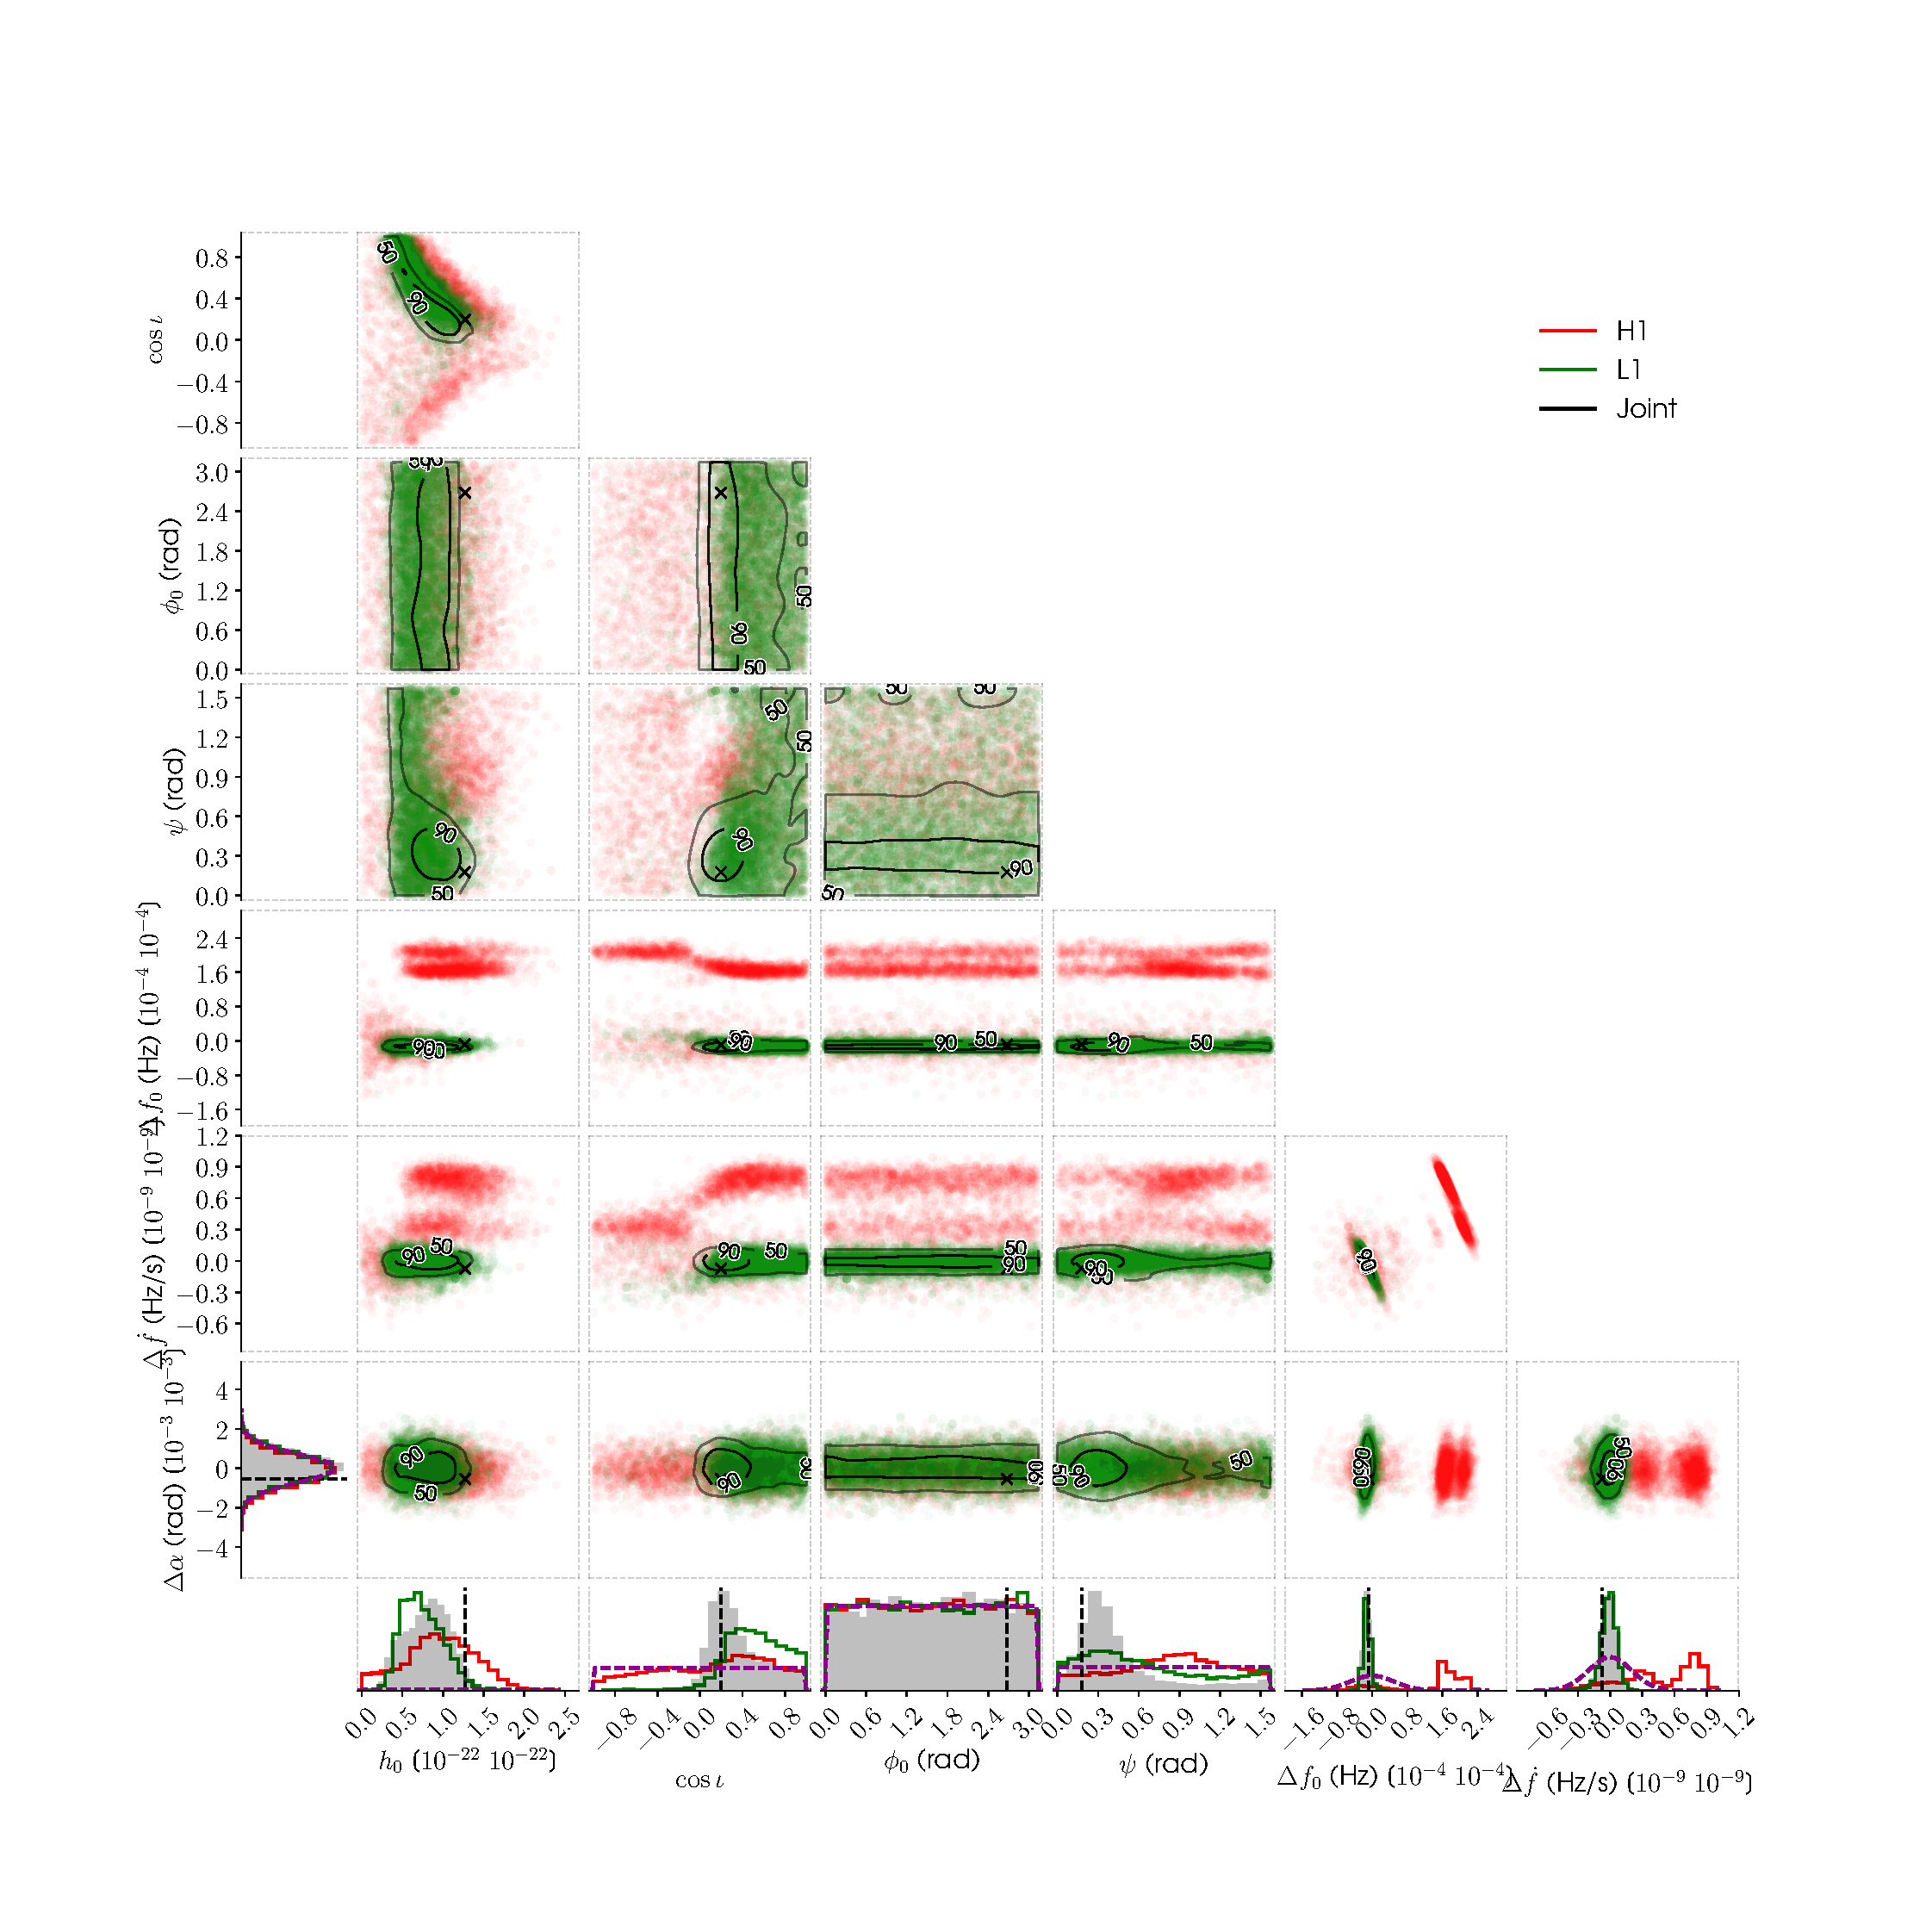
\includegraphics[width=1\columnwidth]{./figures/codeeval/simulations/signal_freq/one/ffdot_inj1}
\caption{ \protect\label{fig:ffdot_inj1}
Posterior probability distributions for the recovered parameters of a simulated signal injected into Gaussian
noise for two LIGO detectors (H1 and L1). The search included the parameters $f_0$, $\dot{f}$, and $\alpha$. The
individual injected SNRs were 4.4 and 6.5 for H1 and L1 respectively, with a coherent SNR of 7.9. The black
vertical dashed lines show the true simulated parameter values, whilst the dashed dark purple lines show the
priors.
}
\end{center}
\end{figure}


\begin{figure}[!phtb]
\begin{center}
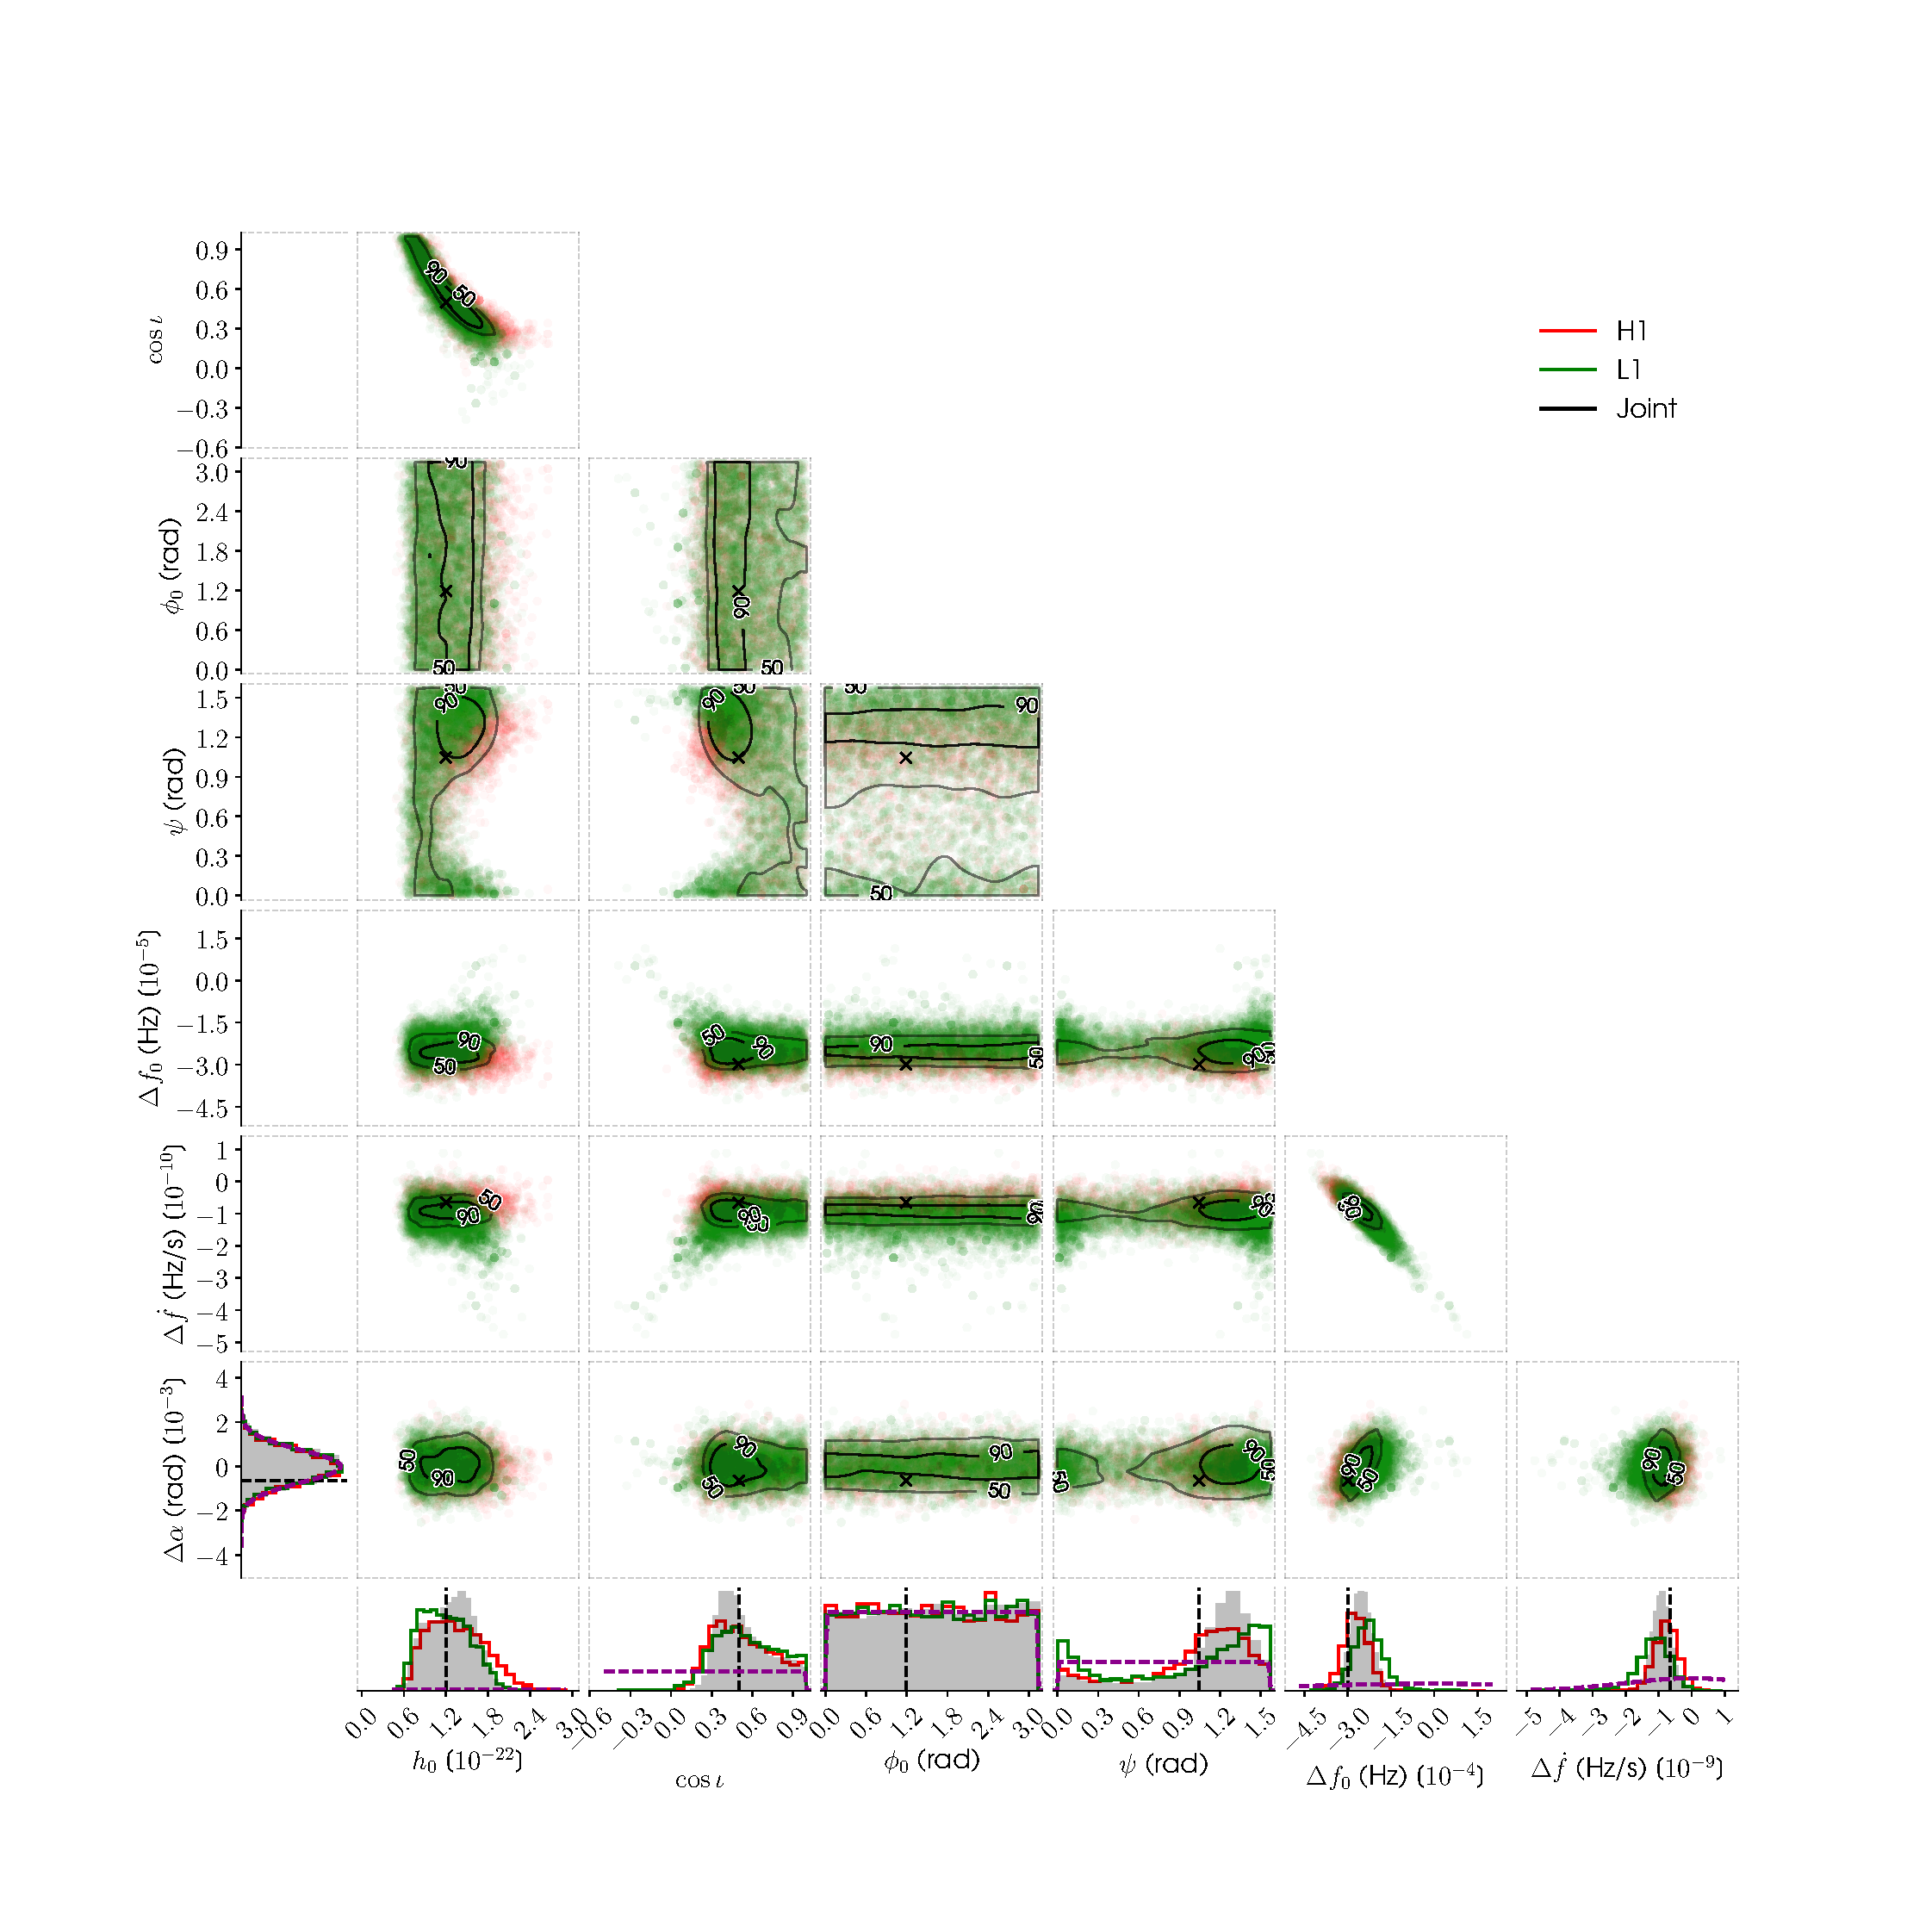
\includegraphics[width=1\columnwidth]{./figures/codeeval/simulations/signal_freq/two/ffdot_inj2}
\caption{ \protect\label{fig:ffdot_inj2}
Posterior probability distributions for the recovered parameters of a simulated signal injected into Gaussian
noise for two LIGO detectors (H1 and L1). The search included the parameters $f_0$, $\dot{f}$, and $\alpha$. The
individual injected SNRs were 7.3 and 8.5 for H1 and L1 respectively, with a coherent SNR of 11.2. The black
vertical dashed lines show the true simulated parameter values, whilst the dashed dark purple lines show the
priors.
}
\end{center}
\end{figure}
